\documentclass[a4paper,11pt]{article}
%\pdfoutput=1 % if your are submitting a pdflatex (i.e. if you have
             % images in pdf, png or jpg format)
\usepackage{graphicx}
\usepackage{jcappub} % for details on the use of the package, please
                     % see the JCAP-author-manual

%\usepackage[T1]{fontenc} % if needed
\usepackage{wrapfig}

\usepackage{float}

\title{One Student One Laptop (OSOL)}


%% %simple case: 2 authors, same institution
 \author{Dennis Goeken}
 \author{and Han Yang}

\affiliation{IKAROS Shared Team, Riverty Group GmbH}

% e-mail addresses: one for each author, in the same order as the authors
\emailAdd{dennis.goeken@riverty.com}
\emailAdd{han.yang@riverty.com}

%\abstract{Abstract...}

\begin{document}
\maketitle
\flushbottom
\listoftables
\listoffigures
\newpage

\section{What is One Student One Laptop(OSOL)?}
One Student One Laptop (OSOL) refurbishes donated, out-of-date IT equipment, including laptops, tablets, flat monitors, mouses, and keyboards. After cleaning and disinfecting the devices, we perform a factory reset. Where possible, we install  \href{https://chromeos.google/products/chromeos-flex/}{ChromeOS Flex} (a lightweight, cloud-based operating system) and a selection of educational content. These refurbished devices are then loaned free of charge to students in developing countries to support their education and personal growth.

\section{Why OSOL?}

\subsection{Education would change one life}
Education is more than just learning facts and skills. It is a transformative process that can change your life and the lives of others. Education can help you discover your passions, develop your talents, and achieve your goals. Education can also empower you to make a positive difference in the world, by contributing to social change, economic growth, and human development.

But not everyone has access to quality education. Millions of people around the world face barriers such as poverty, discrimination, conflict, and lack of resources. These challenges prevent them from reaching their full potential and fulfilling their purpose.\cite{education-change-life-world}

\subsubsection{What is Education and Why is it Important?}

Education is the process of acquiring knowledge, skills, values, and attitudes that enable people to learn, grow, and thrive. Education can take many forms, such as formal schooling, informal learning, vocational training, lifelong learning, etc. Education can also cover various subjects, such as literacy, numeracy, science, arts, culture, etc.

Education is important for many reasons. Here are some of them:

\begin{itemize}
	\item \textbf{Education can improve your health and well-being.}
	 Studies have shown that education can reduce the risk of diseases, increase life expectancy, improve mental health, and enhance self-esteem.
	\item \textbf{Education can increase your income and employment opportunities.} 
	 Studies have shown that education can boost your productivity, creativity, and innovation. Education can also help you access better jobs, earn higher wages, and escape poverty.
	\item \textbf{Education can enhance your social and civic participation.} 
	 Studies have shown that education can foster your critical thinking, communication, and collaboration skills. Education can also help you develop your values, beliefs, and identity. Education can also enable you to participate in democratic processes, such as voting, volunteering, and activism.
	\item \textbf{Education can promote peace and justice.}
	 Studies have shown that education can reduce violence, conflict, and extremism. Education can also help you understand different perspectives, respect diversity, and promote human rights.
\end{itemize}

\subsubsection{How Education Can Empower Individuals and Communities}

Education is not only beneficial for individuals but also for communities. Education can empower people to take charge of their own lives and contribute to the common good. Here are some examples of how education can empower individuals and communities:

\begin{itemize}
	\item \textbf{Education can empower children and youth.}
	 Children and youth are the future of our society. They have the potential to shape the world for the better. But they also face many challenges, such as malnutrition, disease, child labor, child marriage, etc. By providing them with education, we can help them grow up healthy, happy, and safe. Education can also help them develop their cognitive, emotional, social, and physical abilities. Education can also enable them to express their opinions, aspirations, and creativity.
	\item \textbf{Education can empower marginalized groups.}
	 Marginalized groups are those who are excluded, ignored or discriminated against because of their ethnicity, religion, disability, sexual orientation, etc. By providing them with education, we can help them overcome these challenges and achieve social inclusion. Education can also help them develop their identity, dignity, and respect. Education can also enable them to access their rights, opportunities, and resources.
	\item \textbf{Education can empower communities.}
	 Communities are groups of people who share a common interest, location, or culture. By providing them with education, we can help them improve their quality of life, well-being, and resilience. Education can also help them develop their social capital, collective action, and problem-solving skills. Education can also enable them to participate in community development, environmental protection, and conflict resolution.
\end{itemize}



\subsection{The Internet and Education} 

The internet has profoundly transformed education, revolutionizing how students learn and access knowledge. Its impact is undeniable, making it an indispensable tool for modern learning.\cite{how-internet-beneficial-students}

The internet provides unparalleled access to a wealth of information, available anytime, anywhere.  Constantly updated content ensures students have access to the most current information, often surpassing the limitations of traditional textbooks. This empowers students to become independent learners, actively engaging with information and taking ownership of their education. Research supports this, demonstrating a correlation between internet access and improved academic performance.\cite{how-much-data-internet-each-day}

However, the digital divide presents a significant challenge. While many students have smartphone access, access to laptops and computers can be limited, particularly in underprivileged households, creating disparities in learning opportunities.  Furthermore, the prevalence of social media among students underscores the need for digital literacy education and responsible internet use.\cite{student-experience-using-internet}

\subsubsection{Unprecedented Access to Information} 

Before the internet, accessing information required significant effort. Libraries and encyclopedias were the primary sources, often limiting access and requiring time-consuming research. The internet has revolutionized this, providing instant access to a vast repository of information, including scholarly articles, research papers, and multimedia resources. This accessibility not only saves time and effort but also fosters independent research and critical thinking skills.\cite{internet-beneficial-students}

\subsubsection{Enhanced Communication and Collaboration}

The internet facilitates seamless communication and collaboration among students, teachers, and educators worldwide. Online platforms enable real-time interaction, enabling students to connect with peers, engage in discussions, and collaborate on projects regardless of geographical location. This fosters a global learning environment, exposing students to diverse perspectives and cultural experiences.\cite{internet-beneficial-students}

\subsubsection{Expanded Access to Educational Resources}

The internet provides access to a wealth of educational resources, including online libraries, interactive learning platforms, and video lectures from renowned experts. These resources enrich the learning experience, offering alternative perspectives, hands-on simulations, and opportunities for in-depth exploration. Students can delve into topics of interest, develop critical thinking skills, and stay abreast of the latest advancements in their fields.

\subsubsection {Online Learning and Certification}

The internet has democratized education by providing access to a wide range of online courses and certification programs offered by prestigious institutions worldwide. These platforms offer flexibility and self-paced learning options, making education more accessible to students with diverse schedules and commitments. Interactive elements, such as quizzes, peer reviews, and discussion forums, enhance the learning experience and foster a sense of community among learners.\cite{importance-reliable-internet-student}

\subsubsection{Flexible Learning Environments}

The internet empowers students to learn anytime, anywhere. No longer confined to traditional classrooms, students can access coursework from the comfort of their homes, libraries, or even while traveling. This flexibility accommodates diverse learning styles and enables students to create personalized learning environments that suit their individual needs and preferences.\cite{importance-reliable-internet-student}

\subsubsection{Beyond the Classroom}

The internet extends the learning experience beyond the classroom. Virtual field trips to museums, historical sites, and scientific laboratories provide immersive experiences, fostering curiosity and broadening horizons. These digital explorations cultivate a sense of global citizenship and empathy, preparing students to thrive in an interconnected world.

\subsubsection{Cost-Effective Learning Opportunities}

The internet has revolutionized access to education by making it more affordable and accessible to a wider audience. Traditional higher education can be expensive, often leaving students with significant debt. The internet offers a compelling alternative, providing high-quality learning opportunities at a fraction of the cost.

For individuals seeking to acquire specific skills or knowledge, the internet is an invaluable resource. Numerous online platforms offer courses on a vast array of subjects, taught by qualified professionals from around the globe. These courses are significantly more affordable than traditional university programs, making education accessible to a broader demographic.

Here are some popular online learning platforms:
\begin {itemize}
	\item \href{https://www.coursera.org/}{Coursera} 
	\item \href{https://www.khanacademy.org/}{Khan Academy} 
	\item \href{https://www.udemy.com/}{Udemy} 
	\item \href{https://www.youtube.com/}{YouTube} 
	\item \href{https://www.edx.org/}{EdX} 
	\item \href{https://www.skillshare.com/}{Skillshare}
\end {itemize}
These platforms cater to diverse learning styles and offer a variety of learning materials, including video lectures, interactive exercises, and quizzes. Many even provide certification upon course completion, enhancing the value proposition for learners.\cite{role-internet-in-education}

\subsection{The Impact of GPT on Education}

Generative pre-trained transformer (GPT) have the potential to revolutionize education in several ways: \cite{ai-in-education}

\subsubsection{Personalized Learning Experiences}

GPT-powered systems can analyze student data, such as learning styles, strengths, and weaknesses, to provide personalized learning experiences. This allows for tailored instruction that adapts to individual needs, optimizing learning outcomes and increasing student engagement.

\subsubsection{24/7 AI-Powered Assistance}

AI-powered chatbots can provide students with on-demand support, answering questions, offering guidance, and providing access to learning materials. This 24/7 availability reduces the burden on teachers and ensures students have timely assistance when needed.

\subsubsection{Enhanced Learning and Reduced Errors}

GPT can assist students in various ways, from identifying and correcting errors in their work to providing constructive feedback. This can help students improve their writing, critical thinking, and problem-solving skills.

\subsubsection{Streamlining Tasks and Fostering Independent Learning}

GPT can help students streamline their tasks, such as summarizing research articles, generating ideas for creative projects, and translating information. This allows students to focus on deeper learning and develop independent learning skills.

\newpage

\section{Related Resources}

\subsection{One Laptop Per Child}
\begin{wrapfigure}{l}{0.5\textwidth}
%	\centering
	
\includegraphics[width=0.5\textwidth]{fig-olpcLogo4}
\end{wrapfigure}

The One Laptop Per Child (OLPC) project was a non-profit initiative that operated from 2005 to 2014 with the ambitious goal of providing every child in the developing world with a rugged, low-cost, low-power laptop computer. \href{https://laptop.org/}{OLPC, Inc} continues to operate, but the design and creation of laptops is no longer part of its mission. \cite{wiki:One_Laptop_per_Child}

\textbf{Key Concepts:}

\begin{itemize}
	\item \textbf{Affordable and Durable:}
	 The core idea was to create a durable and affordable laptop specifically designed for children in developing countries, often lacking access to electricity and reliable internet.
	\item \textbf{Educational Focus:}
	 The project aimed to transform education by providing children with access to information, fostering creativity, and enabling collaborative learning.
	\item \textbf{Community-Driven:}
	 OLPC emphasized community involvement, encouraging children to learn from each other and use technology to solve local problems.
\end{itemize}

\textbf{The XO Laptop:}

A key aspect of the project was the development of the XO laptop, a unique device featuring:
\begin{itemize}
	\item \textbf{Low-power consumption:}
	 Designed to run on minimal energy, often utilizing solar power or hand cranks.
	\item \textbf{Durability:}
	 Built to withstand harsh conditions and rough handling.
	\item \textbf{Educational software:}
	 Pre-loaded with educational software and designed for intuitive use.
	\item \textbf{Connectivity:}
	 Incorporated features like mesh networking to allow laptops to connect and share data even without internet access.
\end{itemize}

\textbf{Impact and Challenges:}

While the OLPC project had a significant impact in some regions, it also faced challenges:
\begin{itemize}
	\item \textbf{High costs:}
	 Achieving the initial goal of a \$100 laptop proved difficult.
	\item \textbf{Sustainability:}
	 Ensuring long-term maintenance and support for the laptops and their software in developing countries presented challenges.
	\item \textbf{Educational impact:}
	 The actual impact on student learning outcomes varied significantly across different regions and implementations.
\end{itemize}

\textbf{Legacy:}

Despite its challenges, the OLPC project has had a lasting impact, inspiring other initiatives focused on providing affordable technology to children in need. It also spurred innovation in low-cost computing and educational technology.


\subsection{World Computer Exchange}
\begin{wrapfigure}{l}{0.5\textwidth}
	\centering
	
\includegraphics[width=0.9\linewidth]{fig-WORLD-COMPUTER-2-300x122}
\end{wrapfigure}

World Computer Exchange (\href{https://worldcomputerexchange.org/}{WCE}) is a nonprofit organization founded in 1999 by Timothy Anderson, headquartered in Hull, Massachusetts. Its mission is to reduce the digital divide for youth in developing countries by providing refurbished computers and educational resources, thereby enhancing communities and promoting environmentally responsible reuse of electronic equipment. 

WCE operates through multiple chapters across the United States and Canada, collecting donated computers, refurbishing them, and preparing them for shipment to schools, libraries, orphanages, and community organizations in developing nations. Volunteers inspect and repair each computer, installing the Ubuntu operating system along with educational materials to facilitate learning, even without internet connectivity. 

The organization has established partnerships with over 900 entities in 81 developing countries, delivering more than 30,000 computers and setting up approximately 2,675 computer labs by 2011. These efforts have connected numerous youth to the internet, providing access to educational content and opportunities. 

WCE also offers programs like eCorps, which recruits volunteers to install computers and provide technical support at partner sites lacking local expertise. Additionally, the Computers for Girls (C4G) initiative focuses on providing technological training and STEM education to girls in countries such as Ghana, Liberia, Mali, Zambia, and Pakistan. 

By refurbishing and distributing computers, WCE not only promotes education and technological skills among youth in developing countries but also contributes to environmental sustainability by preventing electronic waste from ending up in landfills. 

According to UNESCO, it is North America's largest non-profit supplier of tested used computers to schools and community organizations in developing countries. \cite{wiki:World_Computer_Exchange}


\subsection{UNESCO}
\begin{wrapfigure}{l}{0.5\textwidth}
	\centering
	
\includegraphics[width=0.9\linewidth]{fig-unesco-logo}
\end{wrapfigure}

Education is fundamental to UNESCO's mission to build a peaceful, equitable, and sustainable world. It is a fundamental human right for all, throughout life. As the UN agency with a mandate covering all aspects of education, UNESCO leads the Global Education 2030 Agenda, striving to achieve Sustainable Development Goal 4.
\cite{unesco-education-transforms-lives}

\subsubsection{The Importance of Digital Innovation in Education}

In today's interconnected world, digital technology is crucial for ensuring equitable access to education. The COVID-19 pandemic starkly highlighted the digital divide, with many students lacking access to reliable internet and quality digital learning resources. This disruption underscored the urgent need to leverage technology to create more inclusive, resilient, and equitable education systems.

UNESCO supports the integration of digital innovation to:
\begin{itemize}
	\item \textbf{Expand access to education:} Bridge the digital divide and ensure equitable access to quality education for all.
	\item \textbf{Enhance learning:} Improve the quality and relevance of learning by leveraging innovative technologies.
	\item \textbf{Foster lifelong learning:} Develop ICT-enhanced pathways for lifelong learning and skill development.
	\item \textbf{Strengthen education systems:} Build robust and resilient education systems that effectively utilize technology.
	\item \textbf{Develop digital literacy:} Equip teachers and students with the necessary digital skills and competencies.
\end{itemize}

\subsubsection{The Role of Artificial Intelligence in Education}

Artificial Intelligence (AI) presents both significant opportunities and challenges for education. While AI has the potential to personalize learning, automate administrative tasks, and improve educational outcomes, it is crucial to ensure that AI applications are inclusive, equitable, and human-centered.

UNESCO supports Member States in harnessing the potential of AI to achieve the Education 2030 Agenda. Key areas of focus include:
\begin{itemize}
	\item \textbf{Addressing inequalities:} Ensuring AI does not exacerbate existing inequalities in access to education and opportunities.
	\item \textbf{Promoting inclusivity:} Ensuring AI technologies are accessible and inclusive for all learners, regardless of their background or abilities.
	\item \textbf{Guiding ethical AI development:} Promoting the ethical and responsible development and use of AI in education.
\end{itemize}

UNESCO's guidance documents, such as \href{https://unesdoc.unesco.org/ark:/48223/pf0000376709}{"Artificial Intelligence and Education: Guidance for Policy-makers"}, provide valuable insights for educators, policymakers, and practitioners on how to effectively and ethically integrate AI into education systems.
\cite{unesco-education-ai}


\section{What OSOL will benfit to Riverty and Bertelsmann?}

Each loaned IT devices features several OSOL stickers prominently displaying the Riverty and Bertelsmann logos, as illustrated in Figure \ref{fig:osol-sticker}. 

\begin{figure}[h!]
	\centering
	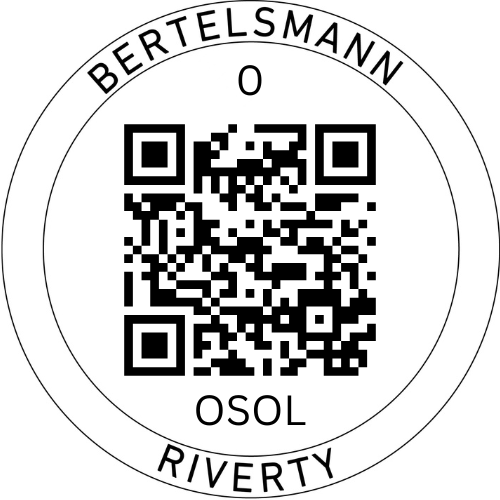
\includegraphics[width=0.7\linewidth]{fig-osol-sticker}
	\caption{OSOL sticker sample}
	\label{fig:osol-sticker}
\end{figure}

The OSOL sticker provides several advertising benefits:
\begin{itemize}
	\item \textbf{Brand Visibility:}
	\begin{itemize}
		\item \textbf{Increased Brand Awareness:} Every device with the sticker acts as a moving advertisement. Wherever the device goes, the logos are visible, increasing brand awareness among the recipients (students) and anyone who comes into contact with the device.
		\item \textbf{Brand Association with Education:} By associating their brands with an initiative that provides educational technology to underprivileged students, both Riverty and Bertelsmann can enhance their corporate social responsibility image. This can positively impact public perception and attract potential customers who value socially conscious companies.
	\end{itemize}
	\item Community Impact:
	\begin{itemize}
		\item \textbf{Positive Brand Perception:} The sticker visibly demonstrates the companies' commitment to supporting education and improving the lives of children in developing countries. This can generate positive goodwill within the communities where the devices are distributed.
	\end{itemize}
	\item Long-Term Exposure:
	\begin{itemize}
		\item \textbf{Sustained Brand Visibility:} The stickers will remain on the devices for an extended period, providing ongoing brand exposure.
	\end{itemize}
	\item Minimal Cost:
	\begin{itemize}
		\item \textbf{Cost-Effective Advertising:} The sticker placement represents a highly cost-effective advertising method compared to traditional advertising channels.
	\end{itemize}
\end{itemize}

The OSOL sticker serves as a low-cost, yet impactful, advertising tool for Riverty and Bertelsmann. It enhances brand visibility, strengthens their corporate social responsibility image, and fosters positive community relations.


\section{How OSOL?}

\subsection{One IT equipment lifecycle}
\begin{figure}[h!]
	\centering
	
\includegraphics[width=0.9\linewidth]{fig-osol-rcc}
	\caption{OSOL equipments lifecycle}
	\label{fig:osol-rcc}
\end{figure}


\subsubsection{Equipment stages}
\begin{enumerate}
	\item Stage 0 - In OSOL Depot
			
	\item Stage 1 - In OSOL Shop
	\begin{itemize}
		\item \textbf{Hardware:}  basic repair, clean, disinfect
		\item\textbf{Software:} factory reset, install ChromeOS Flex, install selected  education content
	\end{itemize}
		
	\item Stage 2 - Distribution to Students
	\begin{itemize}
		\item \textbf{less Grade6 or 12 years old:} Tablet
		\item \textbf{from Grade7 or 13 years old)} Laptop
	\end{itemize}
	
	\item Stage 3 - At  Reiverty Computer Center (RCC)
\end{enumerate}	

\subsubsection{Equipment score}
	\begin{itemize}
		\item Each device will have some integer score, which express this device performance and usability.
		\item Each model (cpu, gpu, laptop, tablet, mouse, keyboard, monitor) will have some score, which express this IT model performance.
		\item The device score is decided by the model score, production date and current equip status.
	\end{itemize}
\subsubsection{Equipment annual check}
	\begin{itemize}
		\item Each year we could decide one device score for each equip\_type, the device which score is less than current-year-score will be disuseed.
		\item The disused deviced will be callbacked and send to Riverty Computer Center (RCC).
	\end{itemize}
\subsection{OSOL 2D barcode on IT equipment}

\subsubsection {Stage0 2D barcode data}

\begin{table}[h!]
\begin{center}
	\begin{tabular}{ | c | c | }
		\hline
		1 & stricker\_print\_id \\ 
		\hline
		2 & equip\_id  \\  
		\hline
		3 & from\_person\_id \\
		\hline
		4 & to\_person\_id \\ 
		\hline
		5 &  action\_id \\  
		\hline
		6 & action\_date \\
		\hline
	\end{tabular}
	\caption{Sticker data \-- stage 0}
	\label{table:sticker_data_stage_0}
\end{center}
\end{table}


\subsubsection {Stage1 2D barcode data}

\begin{table}[h!]
	\begin{center}
		\begin{tabular}{ | c | c | }
			\hline
			1 & stricker\_print\_id \\ 
			\hline
			2 & equip\_id  \\  
			\hline
			3 & from\_person\_id \\
			\hline
			4 & to\_person\_id \\ 
			\hline
			5 &  action\_id \\  
			\hline
			6 & action\_date \\
			\hline
			7 &  equip\_score \\  
			\hline
			8 & equip\_info $*$ \\
			\hline
		\end{tabular}
		\caption{Sticker data \-- stage 1}
		\label{table:sticker_data_stage_1}
	\end{center}
\end{table}


If equipment is moniter, equip\_info $*$ is Table \ref{table:sticker_data_stage_1_equip_info_monitor} 
\begin{table}[h!]
	\begin{center}
		\begin{tabular}{ | c | c | }
			\hline
			1 & brand \\ 
			\hline
			2 & model  \\  
			\hline
			3 & release\_date \\
			\hline
			4 & monitor\_type \\ 
			\hline
			5 &  monitor\_resolution \\  
			\hline
			6 & vga \\
			\hline
			7 &  dvi \\  
			\hline
			8 & dp \\
			\hline
			9 & hdmi \\
			\hline
			10 & usb\_c \\  
			\hline
			11 & production\_date \\
			\hline
		\end{tabular}
		\caption{Sticker data \-- stage 1 \-- equip\_info $*$ \-- monitor}
		\label{table:sticker_data_stage_1_equip_info_monitor}
	\end{center}
\end{table}

If equipment is keyboard, equip\_info $*$ is Table \ref{table:sticker_data_stage_1_equip_info_keyboard}
\begin{table}[h!]
	\begin{center}
		\begin{tabular}{ | c | c | }
			\hline
			1 & brand \\ 
			\hline
			2 & model  \\  
			\hline
			3 & release\_date \\
			\hline
			4 & is\_wireless \\ 
			\hline
			5 &  is\_bluetooth \\  
			\hline
			6 & is\_usb\_receiver \\
			\hline
			7 &  key\_number \\  
			\hline
			8 & keyboard\_type \\
			\hline
			9 & production\_date \\
			\hline
		\end{tabular}
		\caption{Sticker data \-- stage 1 \-- equip\_info $*$ \-- keyboard}
		\label{table:sticker_data_stage_1_equip_info_keyboard}
	\end{center}
\end{table}


If equipment is mouse, equip\_info $*$ is Table \ref{table:sticker_data_stage_1_equip_info_mouse}
\begin{table}[h!]
	\begin{center}
		\begin{tabular}{ | c | c | }
			\hline
			1 & brand \\ 
			\hline
			2 & model  \\  
			\hline
			3 & release\_date \\
			\hline
			4 & is\_wireless \\ 
			\hline
			5 &  is\_bluetooth \\  
			\hline
			6 & is\_usb\_receiver \\
			\hline
			7 & production\_date \\
			\hline
		\end{tabular}
		\caption{Sticker data \-- stage 1 \-- equip\_info $*$ \-- mouse}
		\label{table:sticker_data_stage_1_equip_info_mouse}
	\end{center}
\end{table}

If equipment is laptop or tablet, equip\_info $*$ is Table \ref{table:sticker_data_stage_1_equip_info_laptop}
\begin{table}[h!]
	\begin{center}
		\begin{tabular}{ | c | c | }
			\hline
			1 & brand \\ 
			\hline
			2 & model  \\  
			\hline
			3 & release\_date \\
			\hline
			4 & cpu\_info $*$ \\ 
			\hline
			5 &  memory­\_type \\  
			\hline
			6 & memory\_size(GB) \\
			\hline
			7 & gpu­\_info $*$ \\  
			\hline
			8 & disk\_type \\
			\hline
			9 & disk\_size(GB) \\
			\hline
			10 & monitor­\_type \\  
			\hline
			11 & monitor\_size(inch) \\ 
			\hline
			12 & monitor\_resolution  \\  
			\hline
			13 & is\_wifi \\
			\hline
			14 & is\_bluetooth \\ 
			\hline
			15 & usb\_a\_num \\  
			\hline
			16 & usb\_c\_num \\
			\hline
			17 & hdmi\_num \\
			\hline
			18 & dp\_num \\  
			\hline
			19 & vga\_num \\  
			\hline
			20 & production\_date \\
			\hline
		\end{tabular}
		\caption{Sticker data \-- stage 1 \-- equip\_info $*$ \-- laptop or tablet}
		\label{table:sticker_data_stage_1_equip_info_laptop}
	\end{center}
\end{table}

The cpu\_info $*$ is Table \ref{table:sticker_data_stage_1_cpu_info}
\begin{table}[h!]
	\begin{center}
		\begin{tabular}{ | c | c | }
			\hline
			1 & cpu\_name \\ 
			\hline
			2 & manufacturer  \\  
			\hline
			3 & cores \\
			\hline
			4 & clock(GHz) \\ 
			\hline
			5 & L3\_cache(MB) \\  
			\hline
			6 & release\_date \\
			\hline
		\end{tabular}
		\caption{Sticker data \-- stage 1 \-- cpu\_info $*$}
		\label{table:sticker_data_stage_1_cpu_info}
	\end{center}
\end{table}

The gpu\_info $*$ is Table \ref{table:sticker_data_stage_1_gpu_info}
\textbf{\begin{table}[h!]
		\begin{center}
			\begin{tabular}{ | c | c | }
				\hline
				1 & gpu\_name \\ 
				\hline
				2 & manufacturer  \\  
				\hline
				3 & gpu\_chip \\
				\hline
				4 & clock(GHz) \\ 
				\hline
				5 & gpu\_memory(MB) \\  
				\hline
				6 & fp32(TFLOPS) \\  
				\hline
				7 & release\_date \\
				\hline
			\end{tabular}
			\caption{Sticker data \-- stage 1 \-- gpu\_info $*$}
			\label{table:sticker_data_stage_1_gpu_info}
		\end{center}
\end{table}}

\subsubsection {Stage2 2D barcode data}

\begin{table}[H]
	\begin{center}
		\begin{tabular}{ | c | c | }
			\hline
			1 & stricker\_print\_id \\ 
			\hline
			2 & equip\_id  \\  
			\hline
			3 & from\_person\_id \\
			\hline
			4 & to\_person\_id \\ 
			\hline
			5 &  action\_id \\  
			\hline
			6 & action\_date \\
			\hline
		\end{tabular}
		\caption{Sticker data \-- stage 2}
		\label{table:sticker_data_stage_2}
	\end{center}
\end{table}


\subsubsection {Stage3 2D barcode data}
\begin{table}[h!]
	\begin{center}
		\begin{tabular}{ | c | c | }
			\hline
			1 & stricker\_print\_id \\ 
			\hline
			2 & equip\_id  \\  
			\hline
			3 & from\_person\_id \\
			\hline
			4 & to\_person\_id \\ 
			\hline
			5 &  action\_id \\  
			\hline
			6 & action\_date \\
			\hline
		\end{tabular}
		\caption{Sticker data \-- stage 3}
		\label{table:sticker_data_stage_3}
	\end{center}
\end{table}


\subsection{OSOL preinstalled education content}
\subsubsection{\href{https://www.desmos.com/}{Math-desmos}}

\subsubsection{\href{https://chatgpt.com/}{OpenAI ChatGPT}}

\subsubsection{\href{https://gemini.google.com/}{Google Gemini}}

\subsubsection{\href{https://www.researchgate.net/}{ResearchGate}}


	
\subsection{OSOL Tracer - OSOL Data Management System}
\subsubsection{OSOL-T Architecture}

The OSOL-T system is an information management system with the following features:
\begin{itemize}
	\item Records can be imported and accessed globally.
	\item Records are imported and retrieved individually via a graphical user interface (GUI).
	\item The OSOL-T GUI is accessible on any device (web, smart devices, etc.).
	\item Time performance is not a critical requirement for OSOL-T.
\end{itemize}
Given these requirements, a MS Azure Serverless architecture (as depicted in Figure \ref{fig:scalable-ecommerce-web-app}) has been chosen for the OSOL-T system.

\begin{figure}[H]
	\centering
	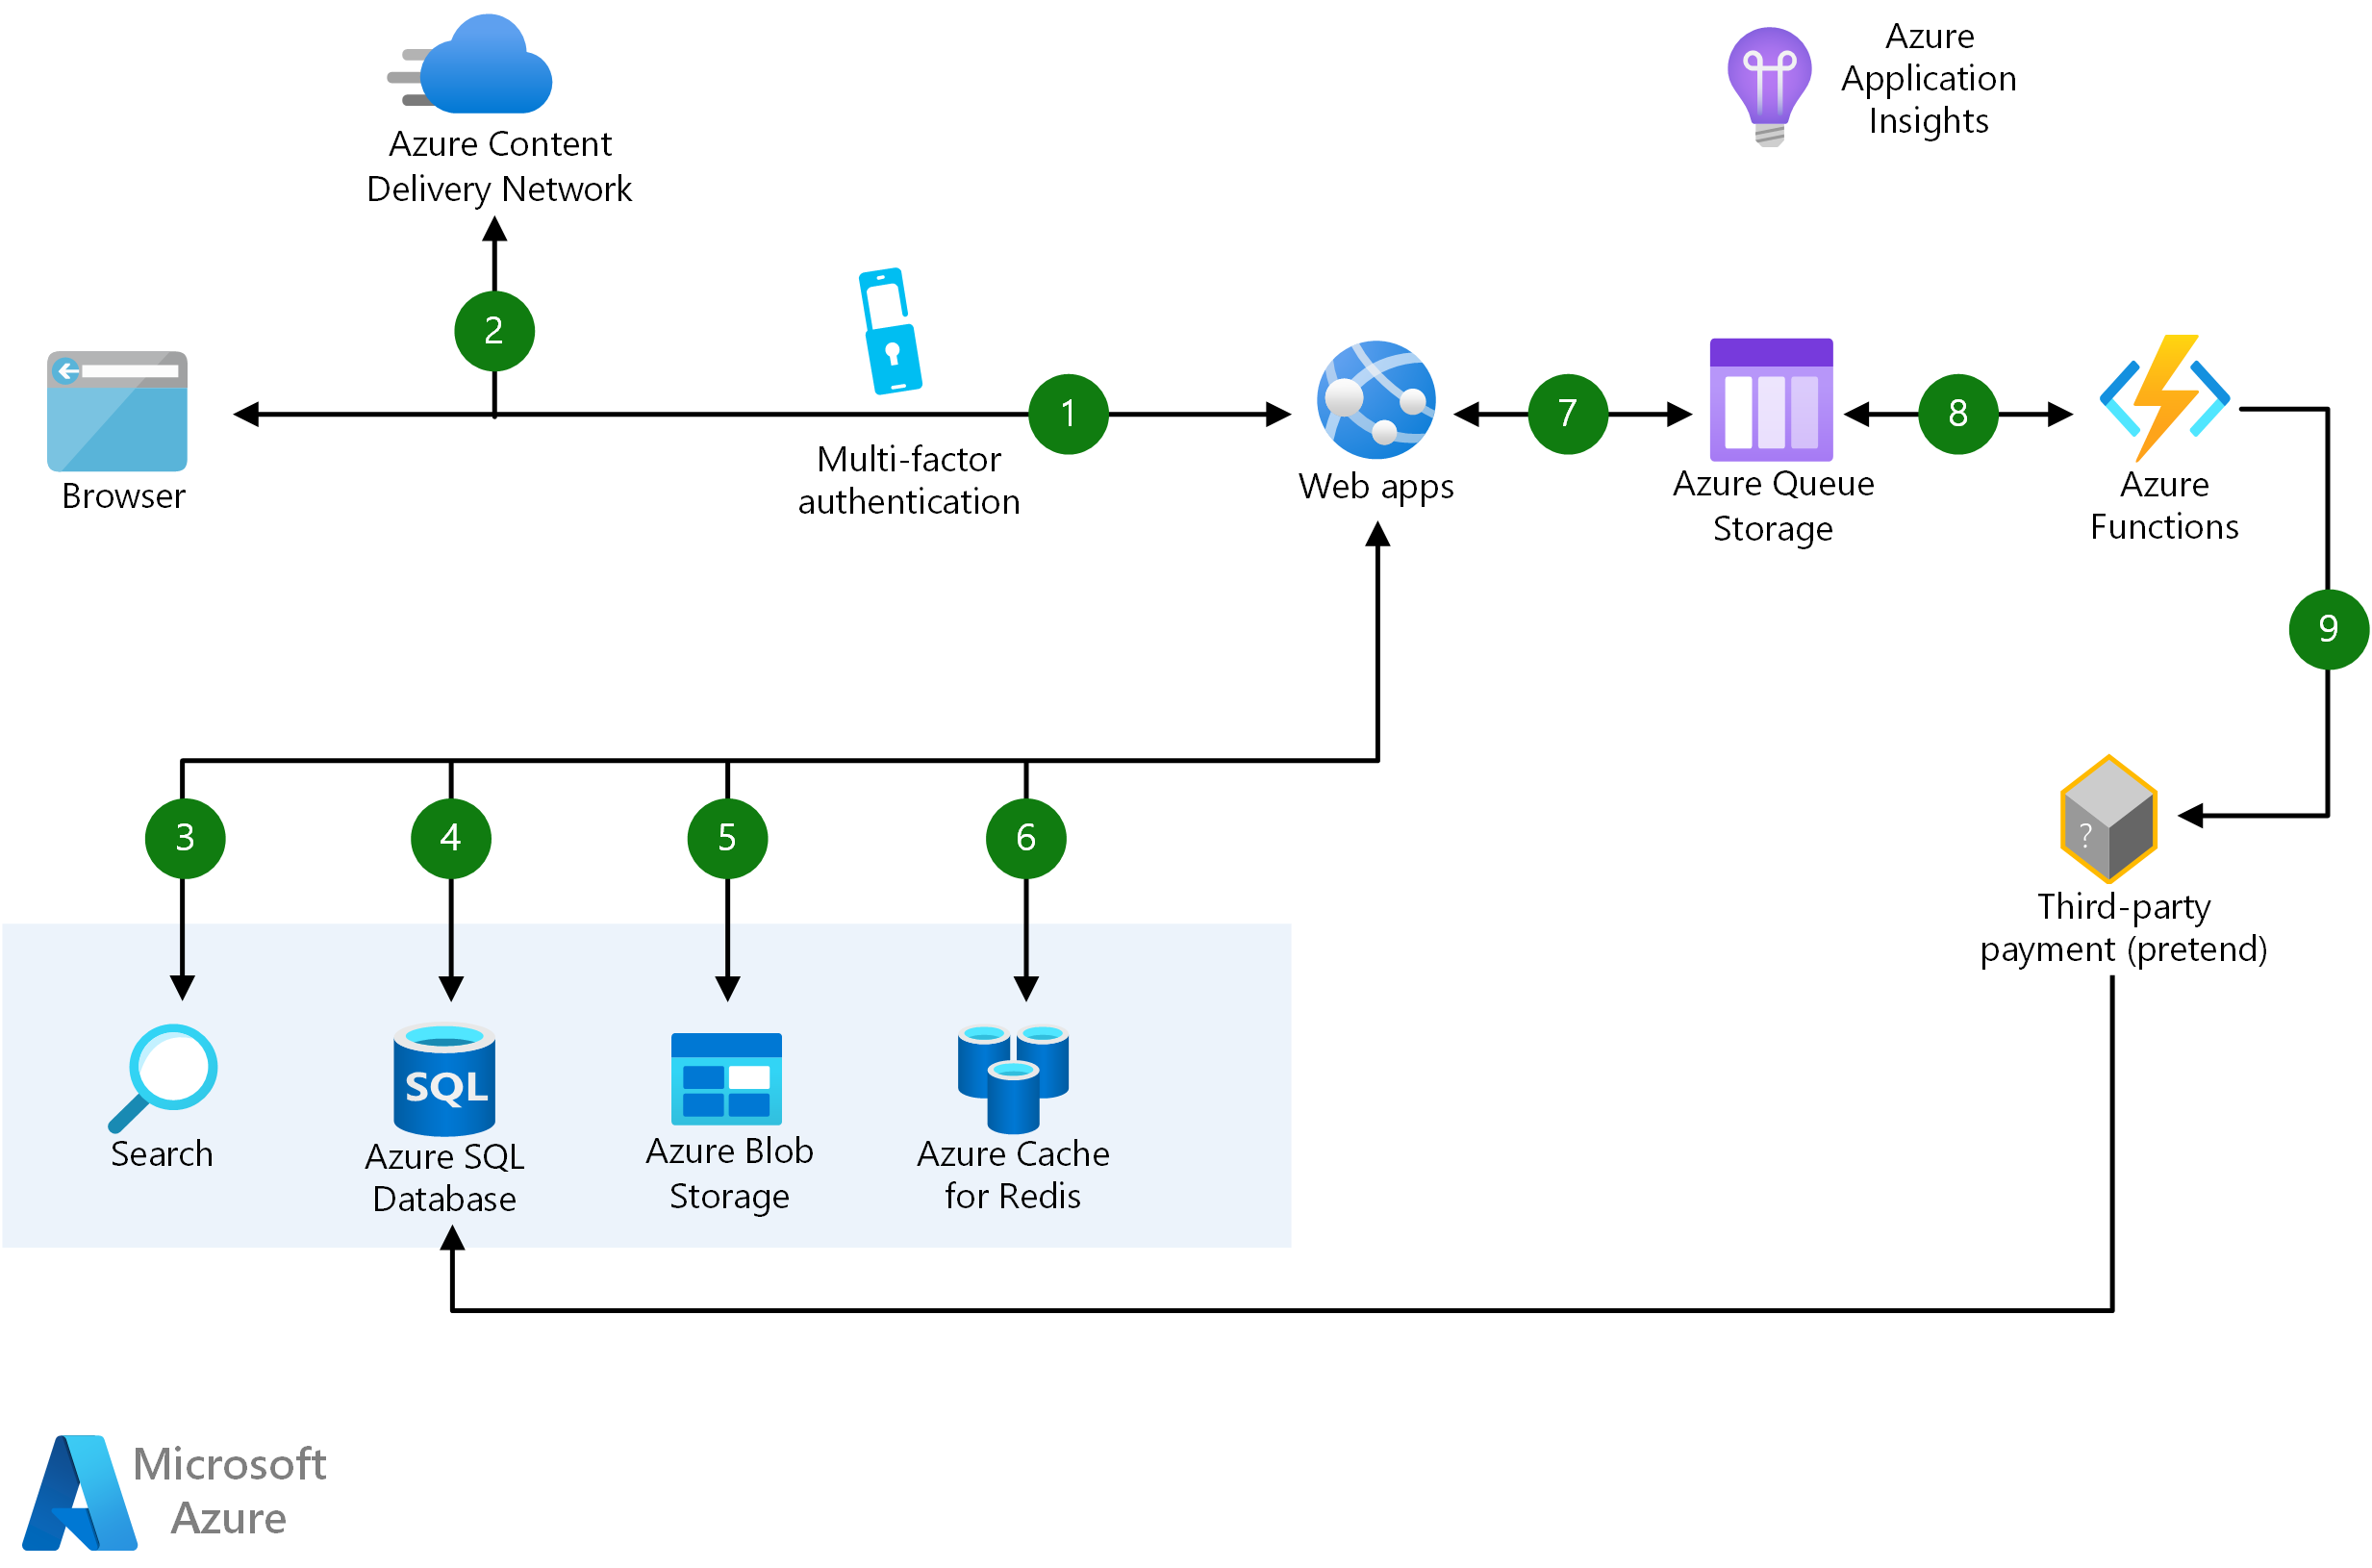
\includegraphics[width=0.65\linewidth]{fig-scalable-ecommerce-web-app}
	\caption{OSOL Tracer system draft architecture\cite{scalable-ecommerce-web-app}}
	\label{fig:scalable-ecommerce-web-app}
\end{figure}


\subsubsection{OSOL-T Database}

\begin{itemize}
	\item OSOL-T database is a relational database.
	\item OSOL-T database will be deployed in MS Azure SQL Server.
\end{itemize}

\begin{figure}[H]
	\centering
	\makebox[\textwidth][c]{
\includegraphics[width=1.2\textwidth]{fig-osol-database}}%
	\caption{OSOL database schema}
	\label{fig:osol-database}
\end{figure}


The OSOL-T database (Figure \ref{fig:osol-database}), detailed in Appendix \ref{appendix-1}, comprises the following tables:
\begin{itemize}
	\item \textbf{osol.person:} Stores records for all individuals associated with the system, including device owners, OSOL staff, students, and RCC staff.  Address and communication information for each person are stored in the related tables:
	\begin{itemize}
		\item \textbf{osol.address}
		\item \textbf{osol.communication}
	\end{itemize}
	\item \textbf{osol.equip:} Contains information on all devices within OSOL, including their current stage and owner.  Device-specific details are stored in the following tables, categorized by equipment type:
	\begin{itemize}
		\item \textbf{osol.laptop}
		\item \textbf{osol.monitor}
		\item \textbf{osol.mouse}
		\item \textbf{osol.keyboard}
	\end{itemize}
	\item \textbf{osol.action:} Records all activities related to a device, such as its entry into OSOL, preparation for lending, lending to a student, return to OSOL, and transfer to RCC.  Associated activity types and possible documents are detailed in the following tables:
	\begin{itemize}
		\item \textbf{conf.action\_type}
		\item \textbf{osol.document}
	\end{itemize}
	\item \textbf{osol.sticker\_print:} Stores information about each printed sticker.  Stickers are printed in relation to a specific action and reflect the device's stage after that action.  Multiple stickers can be printed for a single action.
\end{itemize}


\subsubsection{OSOL-T API}
\begin{itemize}
	\item OSOL-T API is Restful API for each database object CRUD operations.
	\item OSOL-T API will be deployed as MS Azure Function 
\end{itemize}

\subsubsection{OSOL-T API Management }
Azure API Management (APIM) is a powerful tool that helps organizations manage and secure their APIs. As showed in Figure \ref{fig:serverless-web-app}, we could use APIM in OSOL-T system.

\begin{enumerate}
	\item \textbf{Centralized API Management:}
	\begin{itemize}
		\item \textbf{Organize and control:} APIM provides a single platform to manage all your APIs, regardless of where they're hosted (Azure, on-premises, other clouds).
		\item \textbf{Simplify complexity:} It acts as a gateway, abstracting the complexities of your backend systems from the outside world.
		\item \textbf{Consistent policies:} Apply consistent security, access control, and usage policies across all your APIs.
	\end{itemize}
	
	\item \textbf{Enhanced Security:}
	\begin{itemize}
		\item \textbf{Protect your APIs:} APIM offers robust security features like authentication, authorization, rate limiting, and threat protection to safeguard your APIs from unauthorized access and attacks.
		\item \textbf{Control access:} Implement fine-grained access control to restrict who can use your APIs and what they can do.
	\end{itemize}
	
	\item \textbf{Improved Developer Experience:}
	\begin{itemize}
		\item \textbf{Easy discovery:} APIM provides a developer portal where developers can easily discover, explore, and learn about your APIs.
		\item \textbf{Self-service:} Developers can access documentation, code samples, and testing tools to quickly integrate with your APIs.
		\item \textbf{Streamlined onboarding:} Simplify the process for developers to start using your APIs.
	\end{itemize}
	
	\item \textbf{Analytics and Monitoring:}
	\begin{itemize}
		\item \textbf{Gain insights:} APIM provides detailed analytics on API usage, performance, and errors, helping you understand how your APIs are being used and identify potential issues.
		\item \textbf{Monitor performance:} Track API performance and availability to ensure your APIs are meeting your service level agreements.
	\end{itemize}
	
	\item \textbf{Monetization:}
	\begin{itemize}
		\item \textbf{Create revenue streams:} If you want to monetize your APIs, APIM allows you to create subscription plans and track usage for billing purposes.
	\end{itemize}
\end{enumerate}

\begin{figure}[h!]
	\centering
	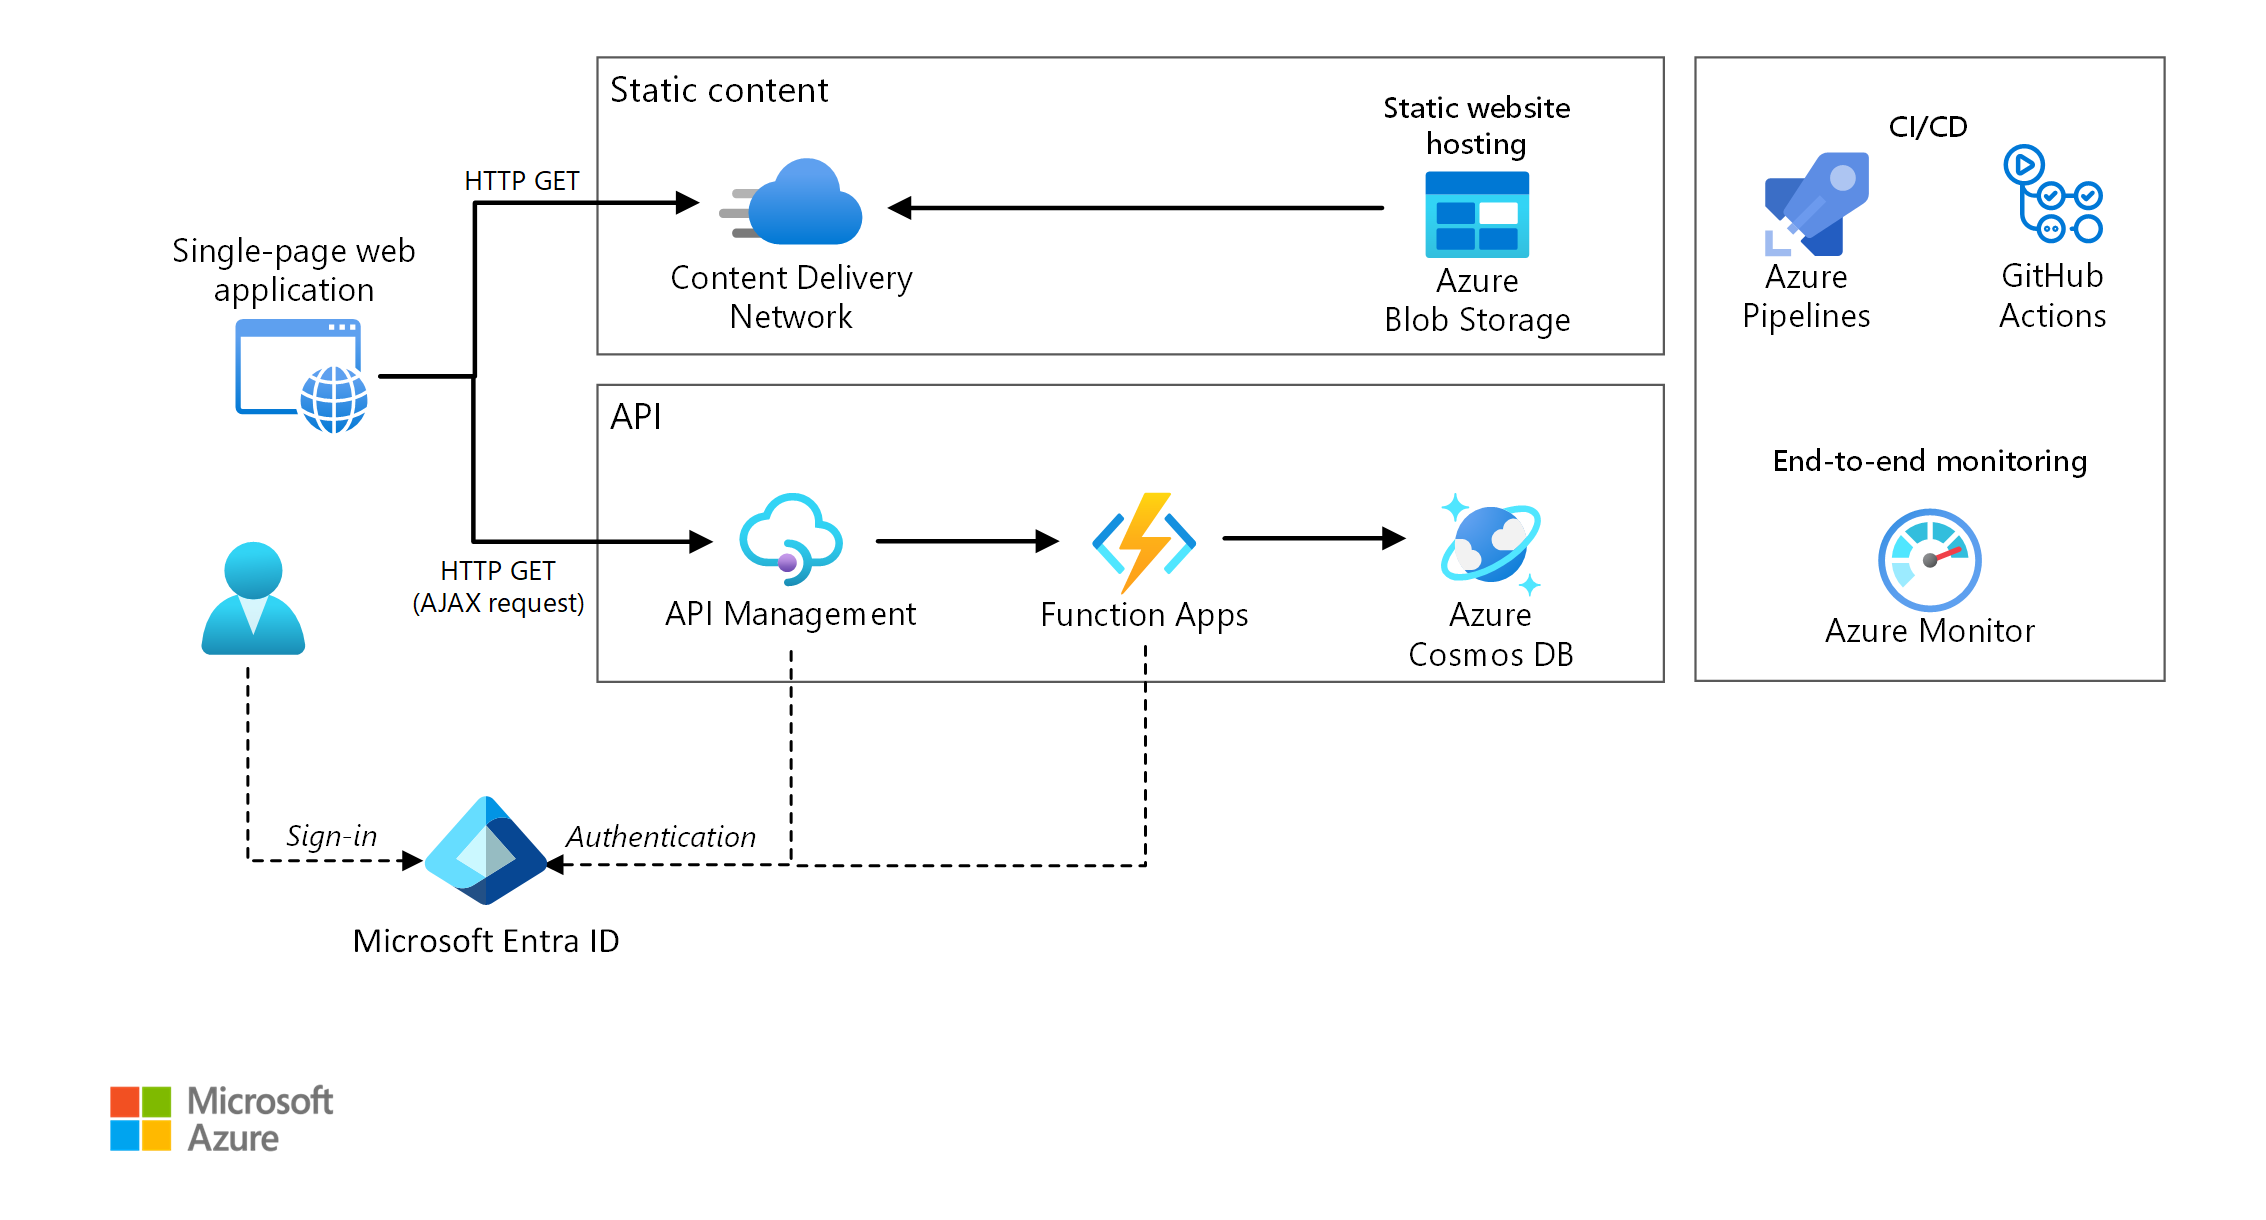
\includegraphics[width=0.9\linewidth]{fig-serverless-web-app}
	\caption{MS Azure Serverless Architecture\cite{serverless-web-app}}
	\label{fig:serverless-web-app}
\end{figure}


\subsubsection{OSOL-T GUI}
OSOL-T GUI include features:
\begin{enumerate}
	\item Multi-Platform - mobile, web - will be implemented with Flutter/Dart
	\item Search
	\item Equip page (CRUD)
	\begin{enumerate}
		\item Laptop page (CRUD)
		\begin{enumerate}
			\item CPU page (CRUD)
			\item GPU page (CRUD)
		\end{enumerate}
		\item Monitor page (CRUD)
		\item Keyboard page (CRUD)
		\item Mouse page (CRUD)
	\end{enumerate}
	\item Person page (CRUD)
	\begin{enumerate}
		\item Address page (CRUD)
		\item Communication page (CRUD) 
	\end{enumerate}
	\item Action page (CRUD)
	\begin{enumerate}
		\item Print equip stage 2D barcode sticker from one action page
	\end{enumerate}
	\item Scan 2D barcode, show data
	\item GPT ChatBot
\end{enumerate}



\subsection{Riverty Computer Center(RCC)}


\section{When OSOL - Schedule}
\subsection{Step 1}
\begin{enumerate}
\item Just one place to store these out-of-date IT equipments.
\item Another guy to monitor and confirm each other with me.
\end{enumerate}

\section{OSOL Budget }

\newpage

\appendix
\section{OSOL-T Database metadata} \label{appendix-1}

\subsection{table\_audit\_columns}
\begin{figure}[H]
	\centering
	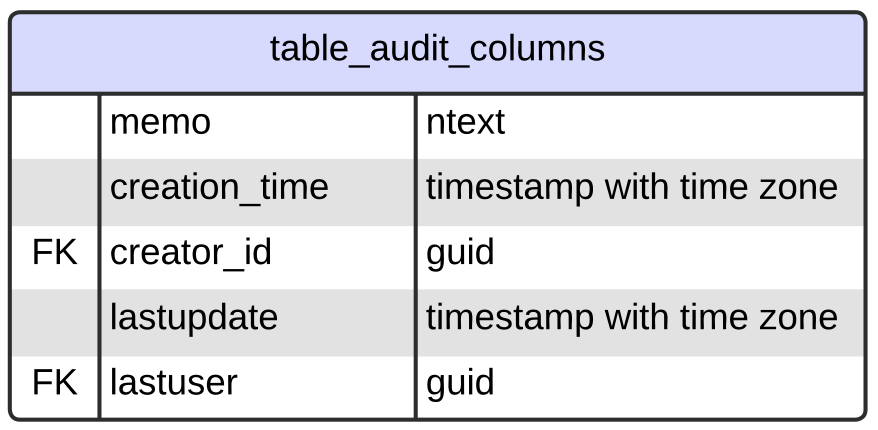
\includegraphics[width=0.5\linewidth]{fig-osol-db-table-audit-columns}
	\caption{OSOL database metadata - table\_audit\_columns}
	\label{fig:osol-db-table-audit-columns}
\end{figure}

\subsection{osol.person}
\begin{figure}[H]
	\centering
	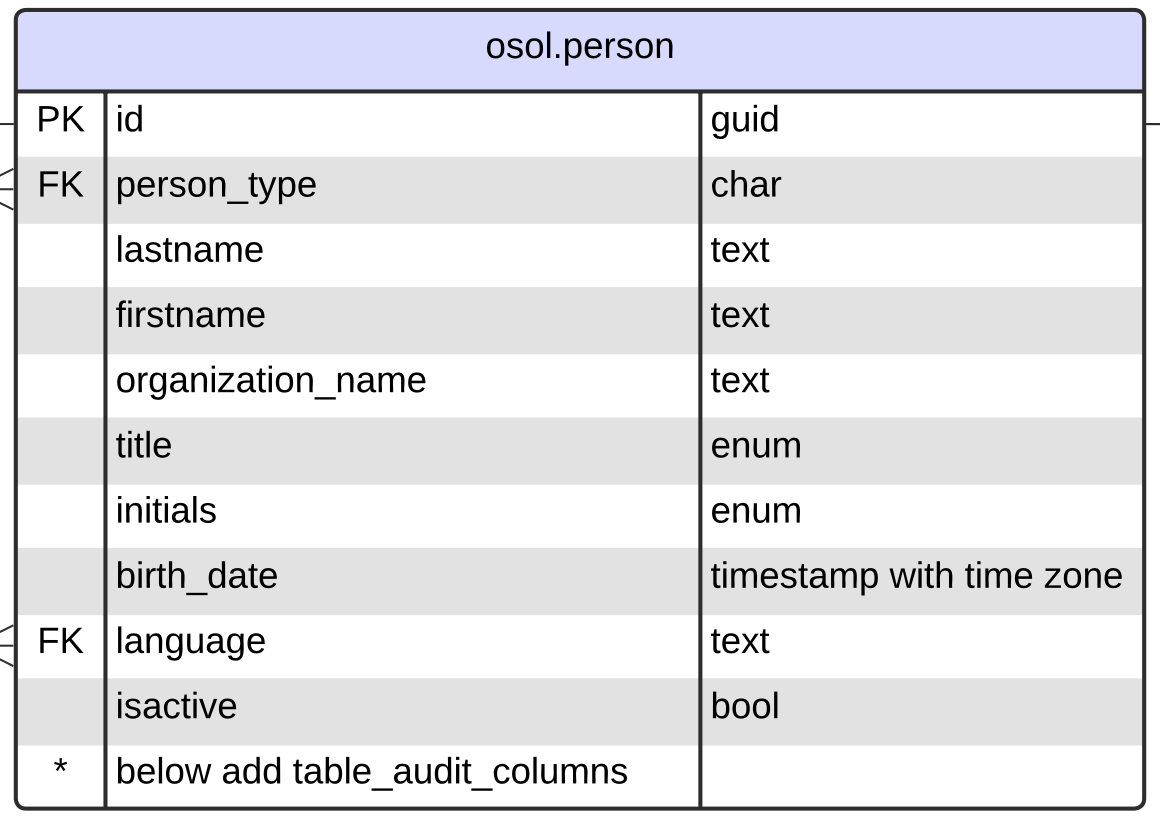
\includegraphics[width=0.6\linewidth]{fig-osol-db-osol-person}
	\caption{OSOL database metadata - osol.person}
	\label{fig:osol-db-osol.person}
\end{figure}

\textbf{title enum:} \{Frau, Frau und Herr, Herr, Miss, Mr, Mrs, Ms \} \\
\textbf{initials enum:} \{Dr., Prof., Prof. Dr.\}

\subsection{conf.person\_type}
\begin{figure}[H]
	\centering
	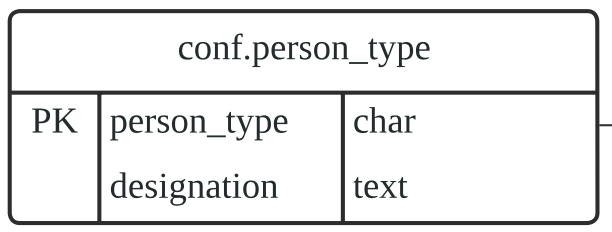
\includegraphics[width=0.4\linewidth]{fig-osol-db-conf-persontype}
	\caption{OSOL database metadata - conf.person\_type}
	\label{fig:osol-db-conf-persontype}
\end{figure}

\begin{table}[h!]
	\begin{center}
		\begin{tabular}{ | c | c | }
			\hline
			\textbf{person\_type} & \textbf{designation} \\
			\hline
			C & company \\ 
			F & female  \\  
			M & male \\
			U & unknown \\ 
			\hline
		\end{tabular}
		\caption{conf.person\_type content}
		\label{table:conf-persontype-content}
	\end{center}
\end{table}

\subsection{conf.language}
\begin{figure}[H]
	\centering
	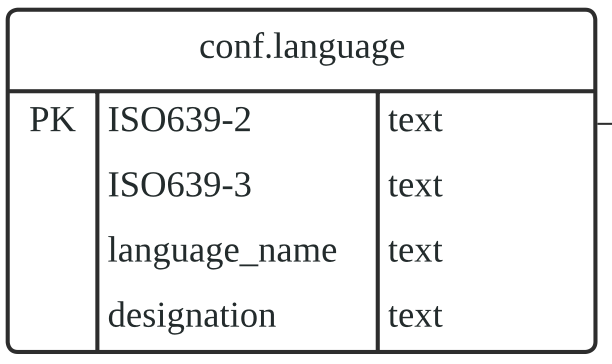
\includegraphics[width=0.4\linewidth]{fig-osol-db-conf-language}
	\caption{OSOL database metadata - conf.language}
	\label{fig:osol-db-conf-language}
\end{figure}

\subsection{osol.address}
\begin{figure}[H]
	\centering
	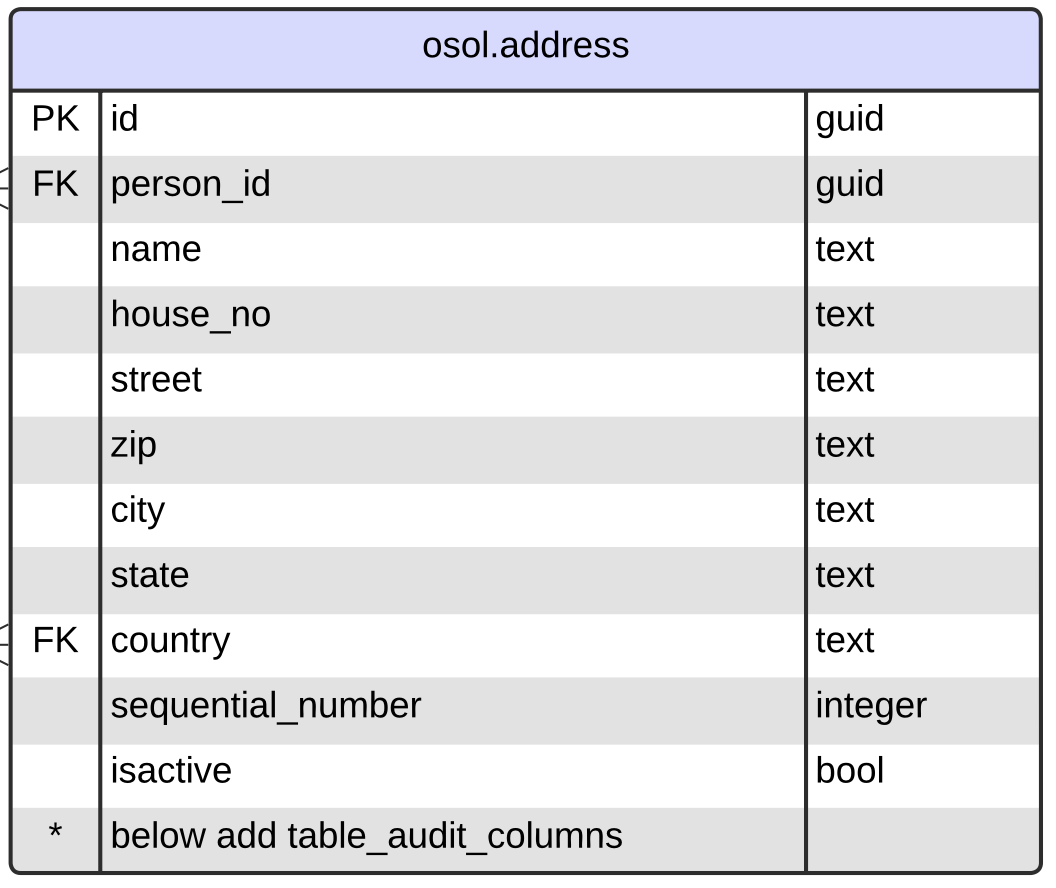
\includegraphics[width=0.6\linewidth]{fig-osol-db-osol-address}
	\caption{OSOL database metadata - osol.address}
	\label{fig:osol-db-osol-address}
\end{figure}

\subsection{conf.country}
\begin{figure}[H]
	\centering
	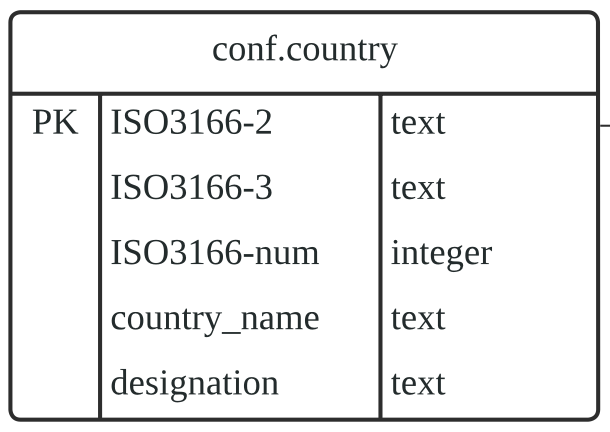
\includegraphics[width=0.4\linewidth]{fig-osol-db-conf-country}
	\caption{OSOL database metadata - conf.country}
	\label{fig:osol-db-conf-country}
\end{figure}

\subsection{osol.communication}
\begin{figure}[H]
	\centering
	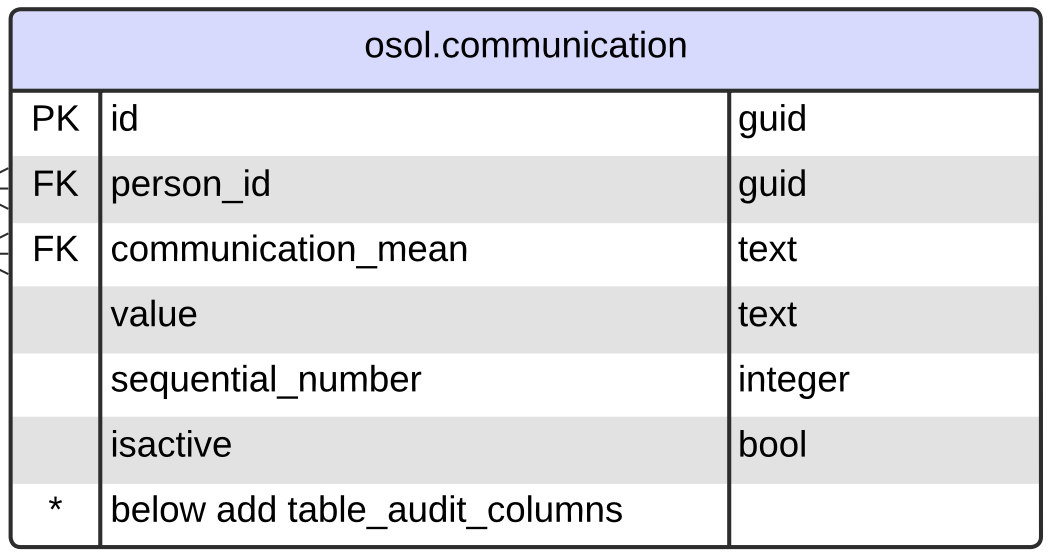
\includegraphics[width=0.6\linewidth]{fig-osol-db-osol-communication}
	\caption{OSOL database metadata - osol.communication}
	\label{fig:osol-db-osol-communication}
\end{figure}

\subsection{osol.communication\_mean}
\begin{figure}[H]
	\centering
	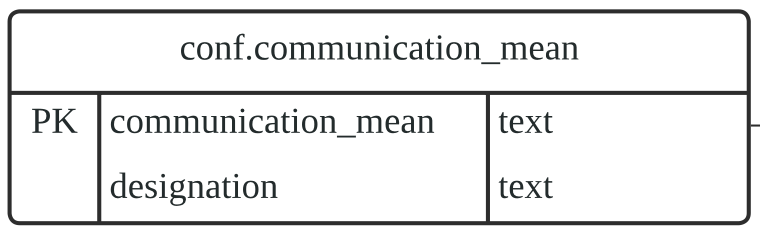
\includegraphics[width=0.4\linewidth]{fig-osol-db-conf-communication-mean}
	\caption{OSOL database metadata - conf.communication\_mean}
	\label{fig:osol-db-conf-communication-mean}
\end{figure}

\begin{table}[h!]
	\begin{center}
		\begin{tabular}{ | c | c | }
			\hline
			\textbf{communication\_mean} & \textbf{designation} \\
			\hline
			telephone & T \\ 
			mobilephone & T  \\  
			fax & T \\
			e-mail & E \\ 
			website &  \\ 
			\hline
		\end{tabular}
		\caption{conf.communication\_mean content}
		\label{table:conf-communication_mean-content}
	\end{center}
\end{table}

\subsection{osol.equip}
\begin{figure}[H]
	\centering
	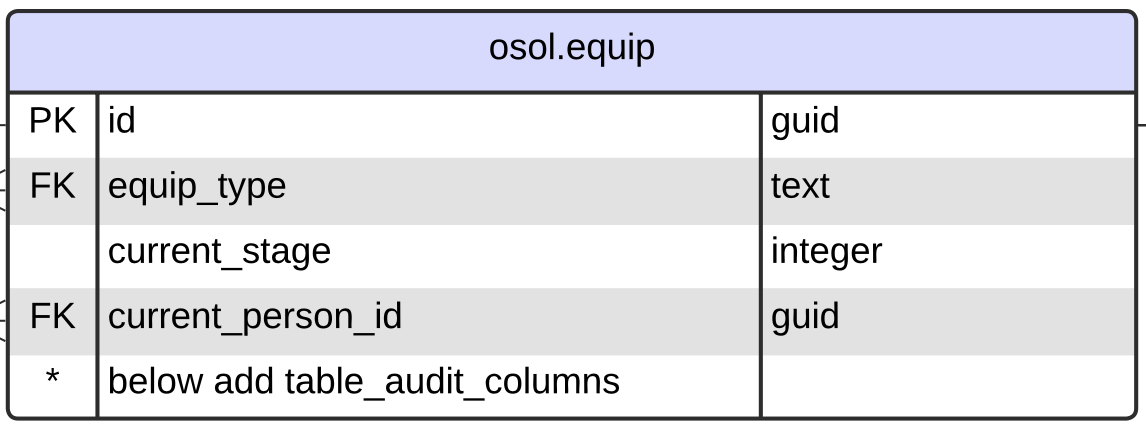
\includegraphics[width=0.6\linewidth]{fig-osol-db-osol-equip}
	\caption{OSOL database metadata - osol.equip}
	\label{fig:osol-db-osol-equip}
\end{figure}

\subsection{conf.equip\_type}
\begin{figure}[H]
	\centering
	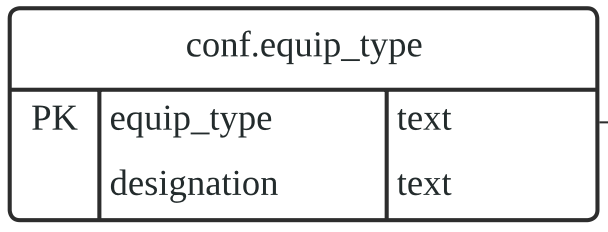
\includegraphics[width=0.4\linewidth]{fig-osol-db-conf-equiptype}
	\caption{OSOL database metadata - conf.equip\_type}
	\label{fig:osol-db-conf-equiptype}
\end{figure}

\begin{table}[h!]
	\begin{center}
		\begin{tabular}{ | c | c | }
			\hline
			\textbf{equip\_type} & \textbf{designation} \\
			\hline
			laptop & desktop or laptop or tablet \\ 
			mouse & mouse  \\  
			keyboard & keyboard \\
			monitor & monitor \\ 
			\hline
		\end{tabular}
		\caption{conf.equip\_type content}
		\label{table:conf-equiptype-content}
	\end{center}
\end{table}

\subsection{osol.monitor}
\begin{figure}[H]
	\centering
	
\includegraphics[width=0.6\linewidth]{fig-osol-db-osol-monitor}
	\caption{OSOL database metadata - osol.monitor}
	\label{fig:osol-db-osol-monitor}
\end{figure}

\subsection{osol.monitor\_model}
\begin{figure}[H]
	\centering
	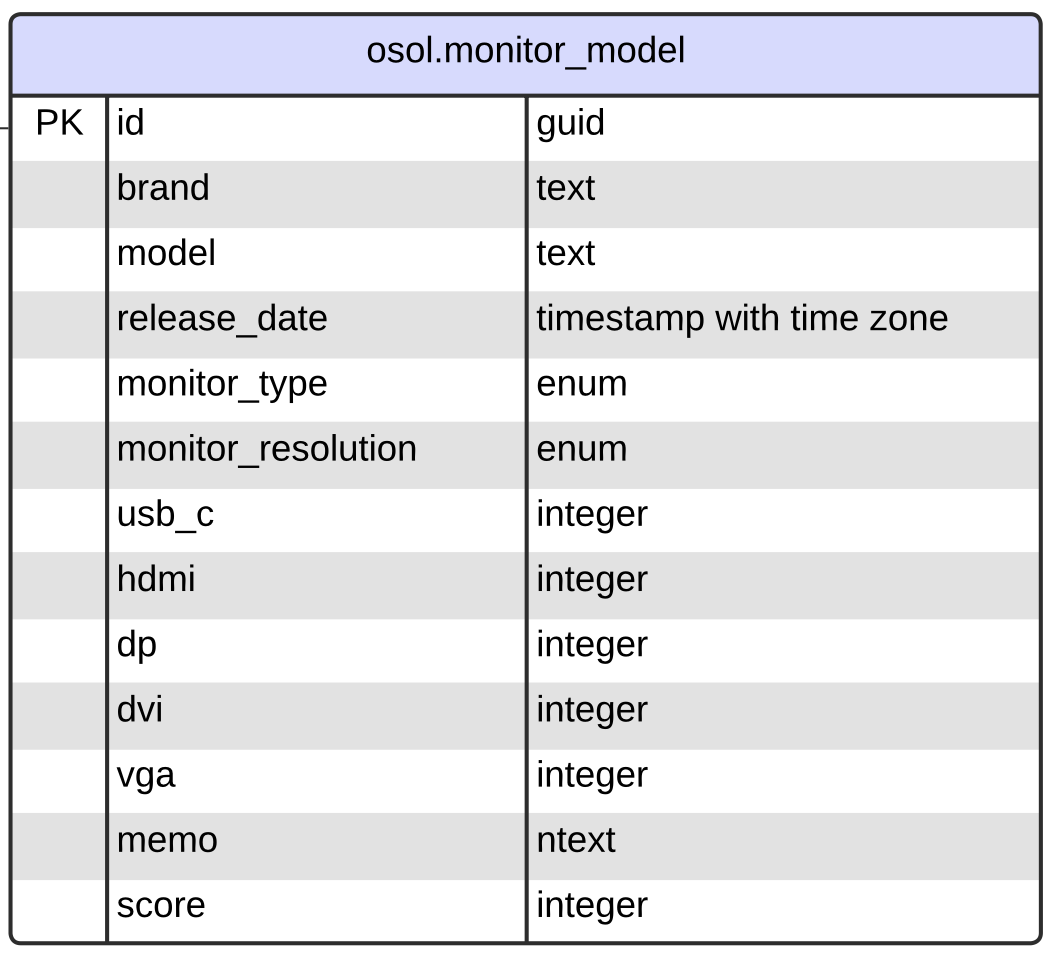
\includegraphics[width=0.6\linewidth]{fig-osol-db-osol-monitor-model}
	\caption{OSOL database metadata - osol.monitor\_model}
	\label{fig:osol-db-osol-monitor-model}
\end{figure}

\textbf{monitor\_type enum:} \{TN, IPS, VA, LED, OLED, QLED\} \\
\textbf{monitor\_resolution enum:} \{1024x768, 1280x720, 1280x800, 1280x1024, 1366x768, 1440x900, 1600x1200, 1920x1080, 2048x1536, 2560x1440, 3840x2160, 5120x2880, 7680x4320\} 

\subsection{osol.keyboard}
\begin{figure}[H]
	\centering
	
\includegraphics[width=0.6\linewidth]{fig-osol-db-osol-keyboard}
	\caption{OSOL database metadata - osol.keyboard}
	\label{fig:osol-db-osol-keyboard}
\end{figure}

\subsection{osol.keyboard\_model}
\begin{figure}[H]
	\centering
	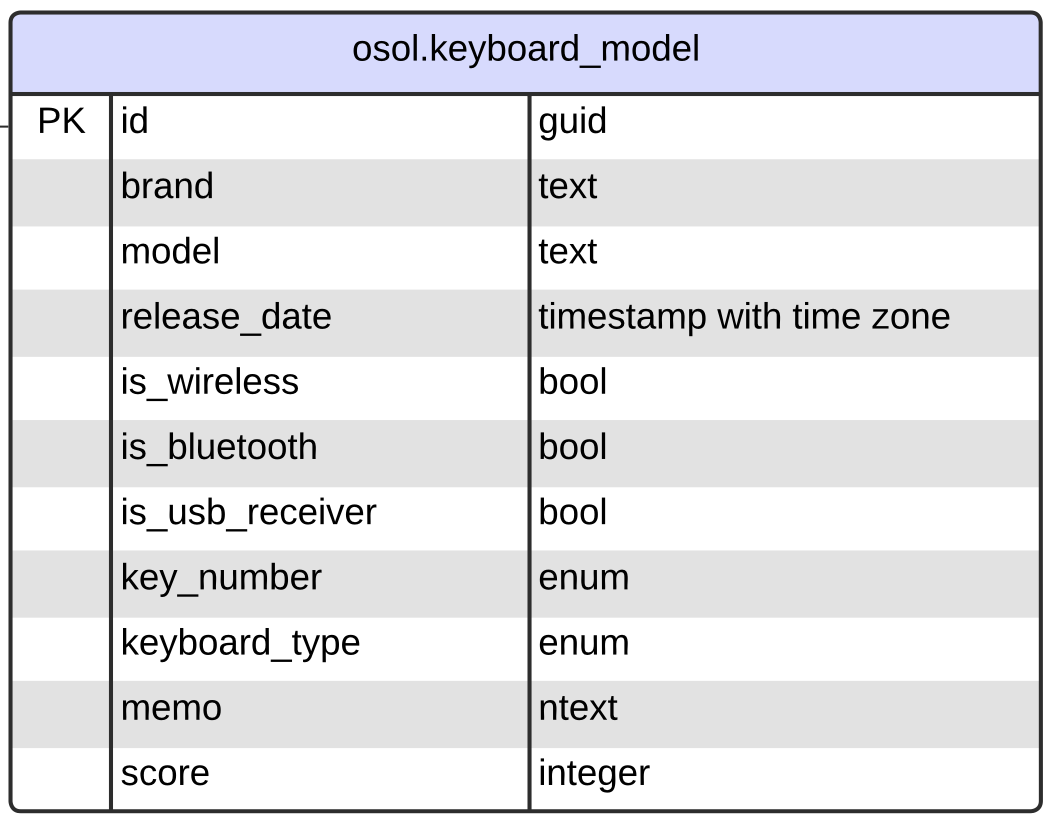
\includegraphics[width=0.6\linewidth]{fig-osol-db-osol-keyboard-model}
	\caption{OSOL database metadata - osol.keyboard\_model}
	\label{fig:osol-db-osol-keyboard-model}
\end{figure}

\textbf{key\_number enum:} \{ \\
\hspace*{2ex} Full-Size Keyboard (104–108 keys), \\
\hspace*{2ex} Tenkeyless (TKL) Keyboard (87–88 keys), \\
\hspace*{2ex} 75\% Keyboard (80–84 keys), \\
\hspace*{2ex} 65\% Keyboard (66–68 keys), \\
\hspace*{2ex} 60\% Keyboard (61 keys)\\
\} \\
\textbf{keyboard\_type enum:} \{Mechanical, Membrane, Scissor-Switch, Optical \& Hall Effect, Capacitive (Topre)\}

\subsection{osol.mouse}
\begin{figure}[H]
	\centering
	
\includegraphics[width=0.6\linewidth]{fig-osol-db-osol-mouse}
	\caption{OSOL database metadata - osol.mouse}
	\label{fig:osol-db-osol-mouse}
\end{figure}

\subsection{osol.mouse\_model}
\begin{figure}[H]
	\centering
	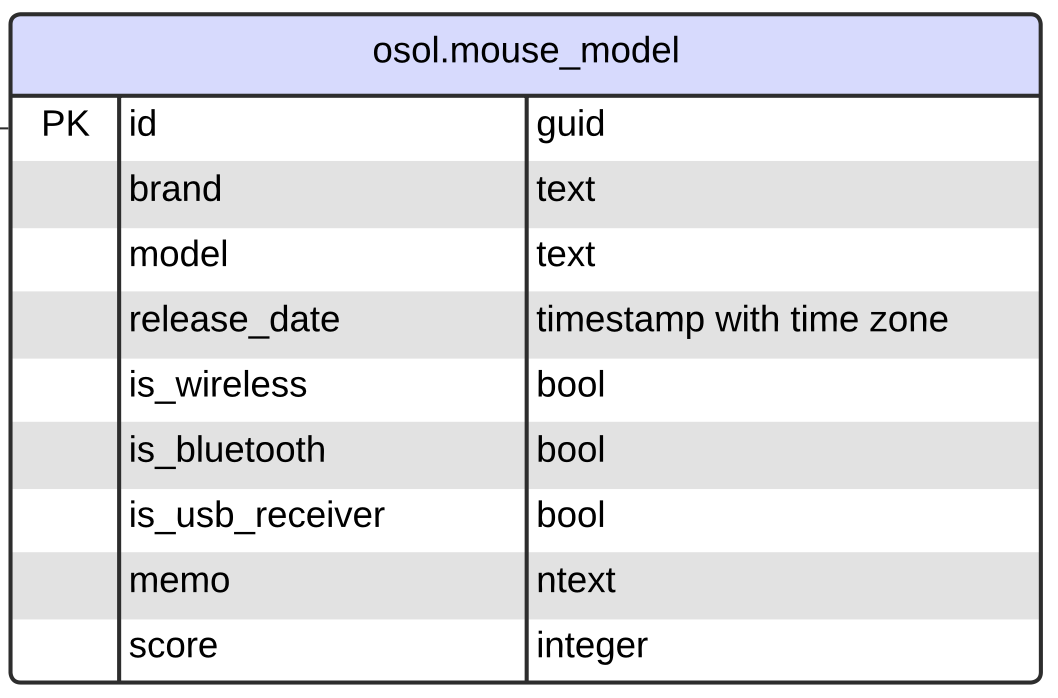
\includegraphics[width=0.6\linewidth]{fig-osol-db-osol-mouse-model}
	\caption{OSOL database metadata - osol.mouse\_model}
	\label{fig:osol-db-osol-mouse-model}
\end{figure}

\subsection{osol.laptop}
\begin{figure}[H]
	\centering
	
\includegraphics[width=0.6\linewidth]{fig-osol-db-osol-laptop}
	\caption{OSOL database metadata - osol.laptop}
	\label{fig:osol-db-osol-laptop}
\end{figure}

\textbf{os enum:} \{ChromeOS Flex, Android, IPadOS\}

\subsection{osol.laptop\_model}
\begin{figure}[H]
	\centering
	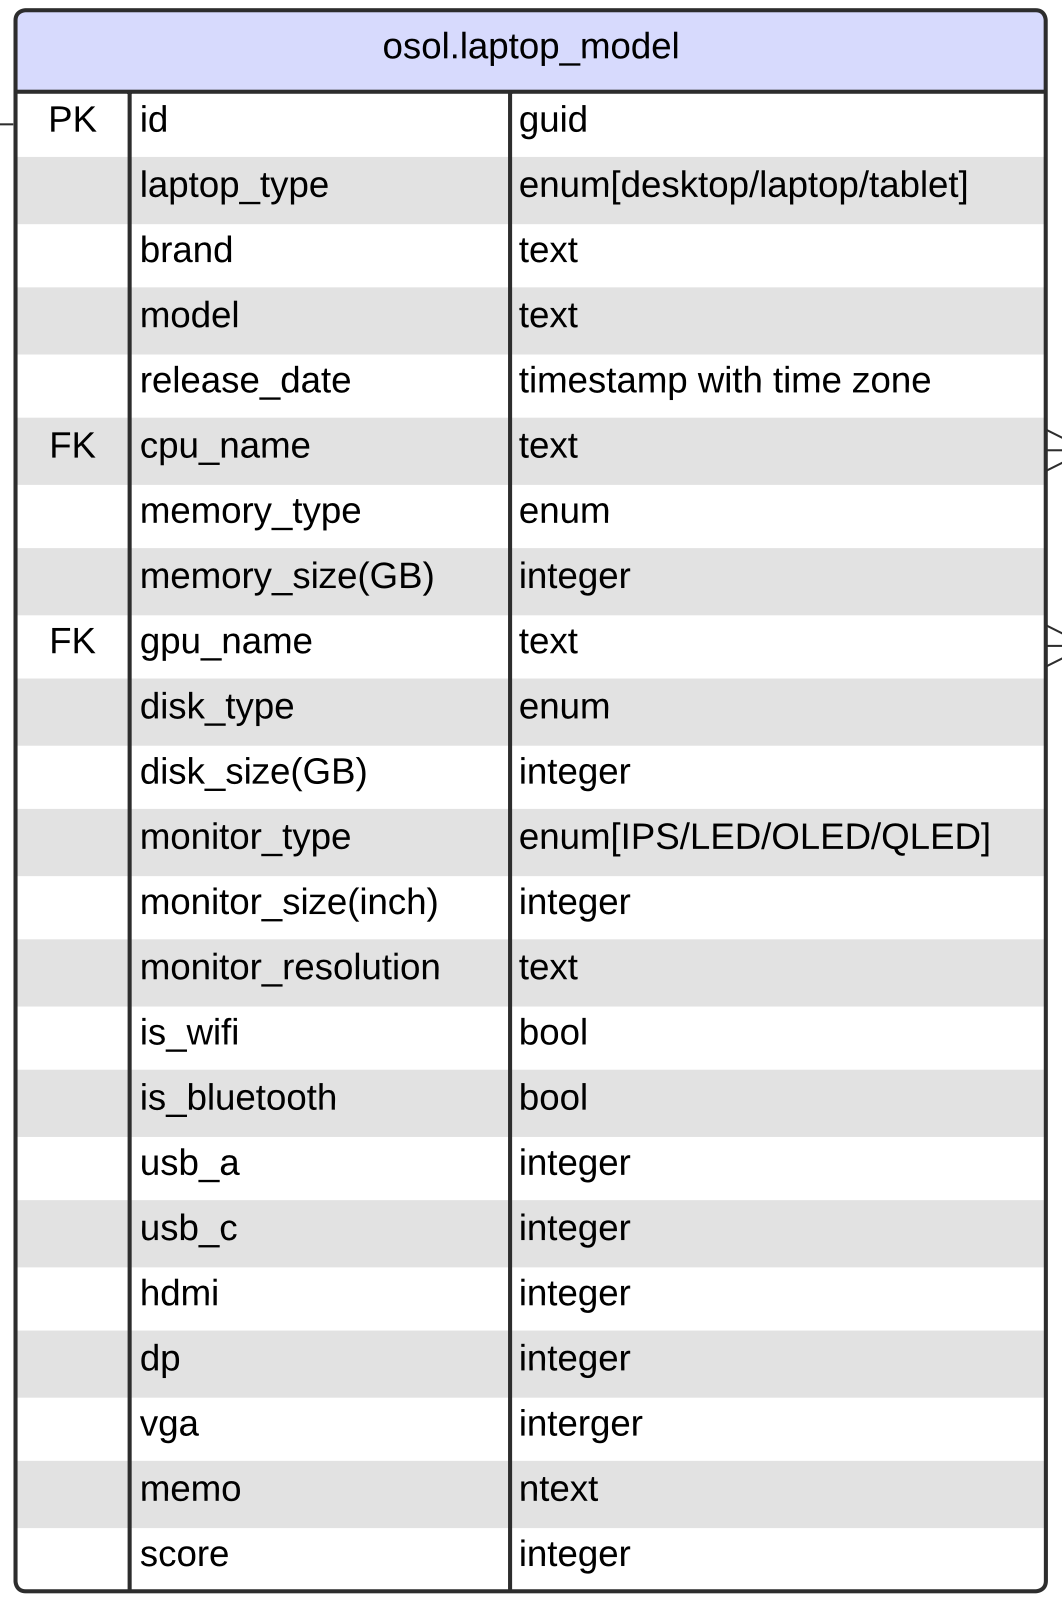
\includegraphics[width=0.6\linewidth]{fig-osol-db-osol-laptop-model}
	\caption{OSOL database metadata - osol.laptop\_model}
	\label{fig:osol-db-osol-laptop-model}
\end{figure}

\textbf{memory\_type enum:} \{DDR3, DDR4, DDR5\} \\
\textbf{disk\_type enum:} \{ \\
\hspace*{2ex} SATA HDD, \\
\hspace*{2ex} SAS HDD, \\
\hspace*{2ex} IDE/PATA HDD, \\
\hspace*{2ex} SATA SSD, \\
\hspace*{2ex} NVMe SSD(PCIeSSD), \\
\hspace*{2ex} M.2 SSD, \\
\hspace*{2ex} U.2 SSD \\
\} \\
\textbf{monitor\_type enum:} \{TN, IPS, VA, LED, OLED, QLED\} 

\subsection{osol.cpu\_model}
\begin{figure}[H]
	\centering
	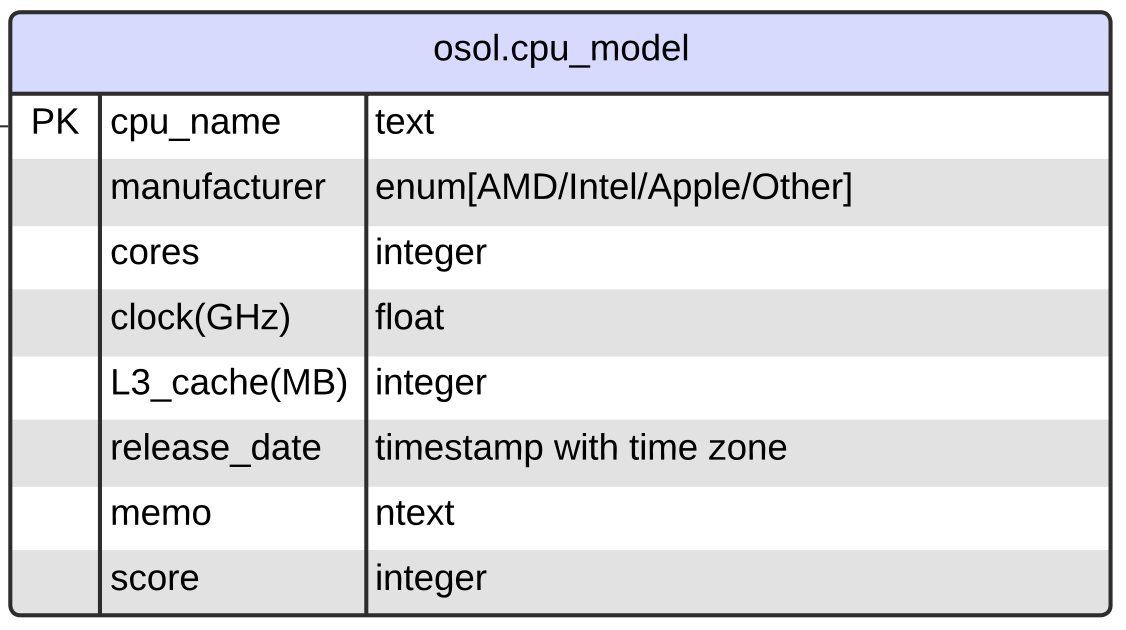
\includegraphics[width=0.6\linewidth]{fig-osol-db-osol-cpu-model}
	\caption{OSOL database metadata - osol.cpu\_model}
	\label{fig:osol-db-osol-cpu-model}
\end{figure}

\textbf{cpu\_model manufacturer enum:} \{AMD, Intel, Apple, Other\}

\subsection{osol.gpu\_model}
\begin{figure}[H]
	\centering
	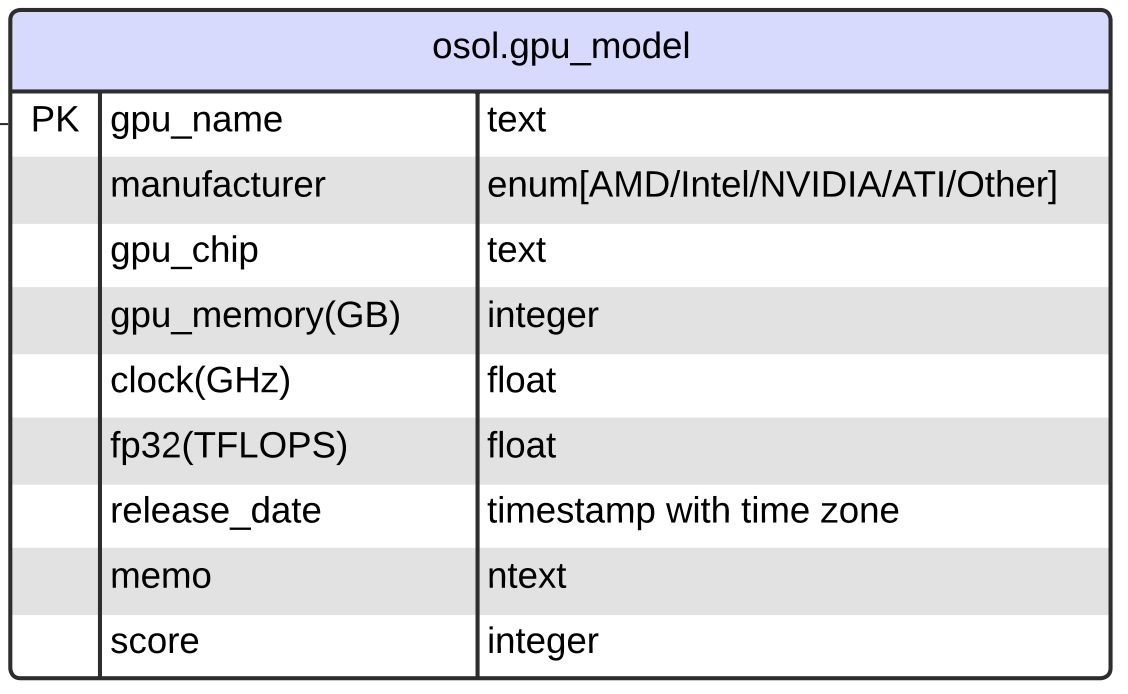
\includegraphics[width=0.6\linewidth]{fig-osol-db-osol-gpu-model}
	\caption{OSOL database metadata - osol.gpu\_model}
	\label{fig:osol-db-osol-gpu-model}
\end{figure}

\textbf{gpu\_model manufacturer enum:} \{AMD, Intel, NVIDIA, ATI, Other\}

\subsection{osol.action}
\begin{figure}[H]
	\centering
	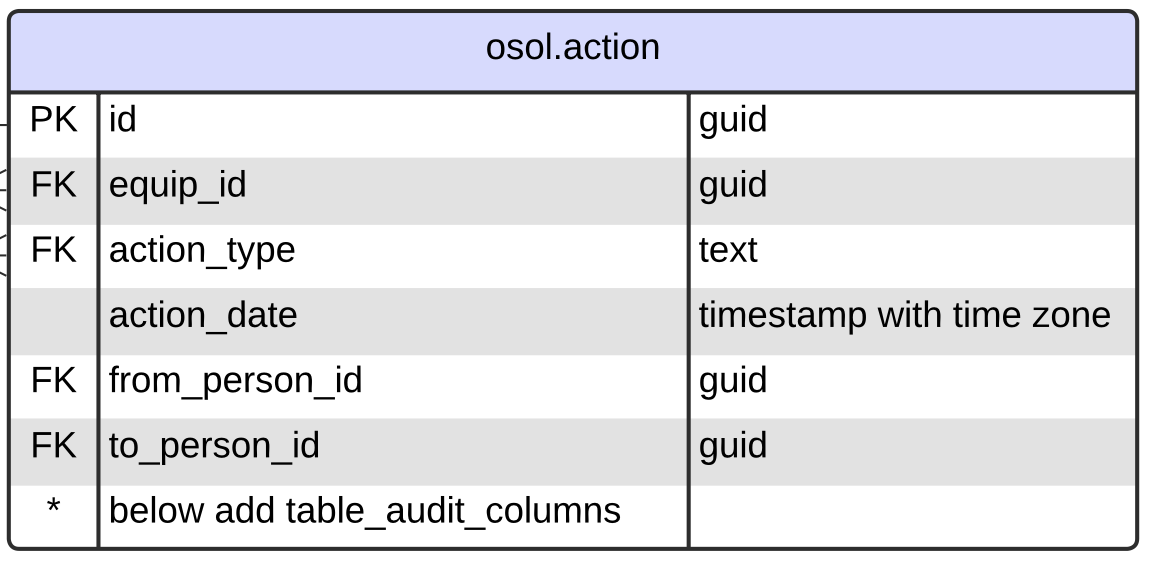
\includegraphics[width=0.6\linewidth]{fig-osol-db-osol-action}
	\caption{OSOL database metadata - osol.action}
	\label{fig:osol-db-osol-action}
\end{figure}

\subsection{osol.action\_type}
\begin{figure}[H]
	\centering
	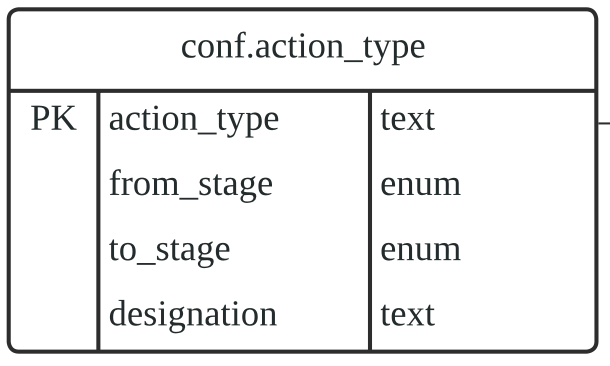
\includegraphics[width=0.4\linewidth]{fig-osol-db-conf-actiontype}
	\caption{OSOL database metadata - osol.action\_type}
	\label{fig:osol-db-osol-action-type}
\end{figure}

\begin{table}[h!]
	\begin{center}
		\begin{tabular}{ | c | c | c | c |}
			\hline
			\textbf{action\_type} & \textbf{from\_stag}e & \textbf{to\_stage} & \textbf{designation} \\
			\hline
			entry & -1 & 0 & \\ 
			prepare & 0 & 1 &   \\  
			lend & 1 & 2 &  \\
			return & 2 & 1 & \\ 
			toRCC & 2 & 3 & \\ 
			comm & & & \\ 
			transfer & & & \\ 
			\hline
		\end{tabular}
		\caption{conf.action\_type content}
		\label{table:conf-actiontype-content}
	\end{center}
\end{table}

\subsection{osol.document}
\begin{figure}[H]
	\centering
	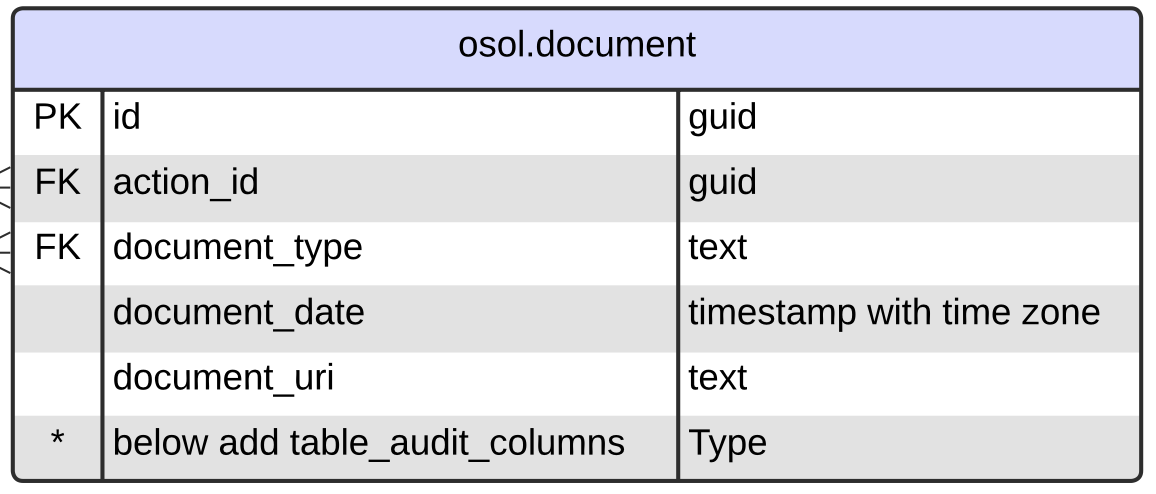
\includegraphics[width=0.6\linewidth]{fig-osol-db-osol-document}
	\caption{OSOL database metadata - osol.document}
	\label{fig:osol-db-osol-document}
\end{figure}

\subsection{osol.document\_type}
\begin{figure}[H]
	\centering
	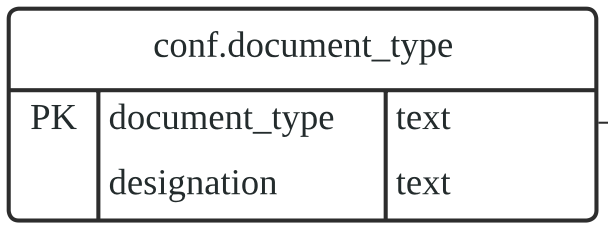
\includegraphics[width=0.4\linewidth]{fig-osol-db-conf-documenttype}
	\caption{OSOL database metadata - osol.document\_type}
	\label{fig:osol-db-osol-document-type}
\end{figure}

\subsection{osol.sticker\_print}
\begin{figure}[H]
	\centering
	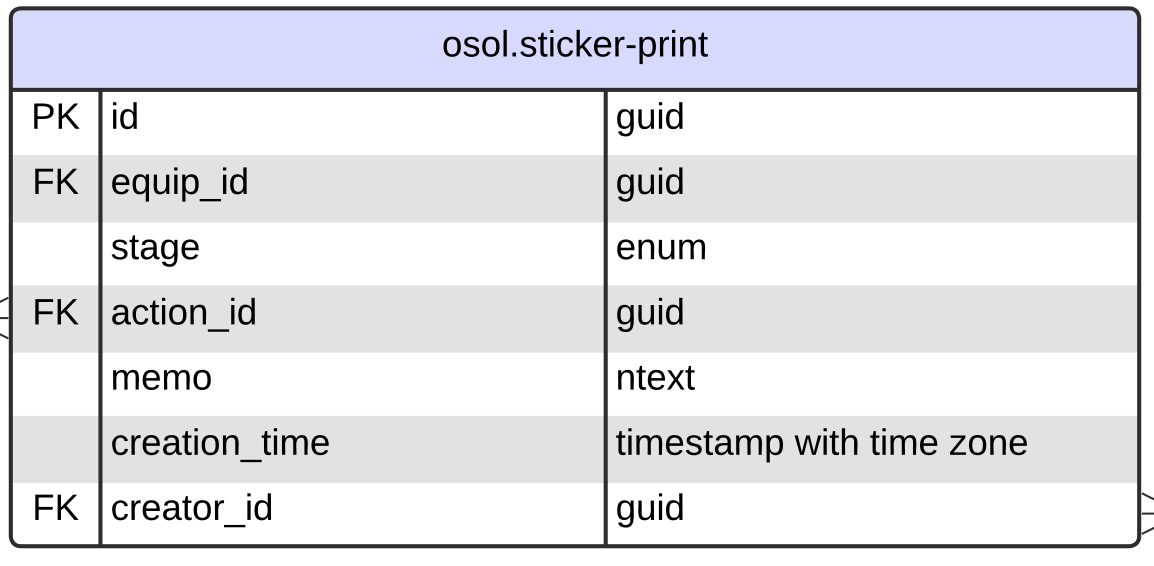
\includegraphics[width=0.6\linewidth]{fig-osol-db-osol-sticker-print}
	\caption{OSOL database metadata - osol.sticker\_print}
	\label{fig:osol-db-osol-sticker-print}
\end{figure}

\newpage

\section{OSOL-T architecture - why use queue?}
\begin{enumerate}
	\item Decoupling
	\begin{itemize}
		\item Purpose: Queues act as a buffer between the API and the downstream services, such as databases or processing logic.
		\item Benefit: This ensures that the API can handle incoming requests without being directly tied to the speed or availability of the downstream services.
		\item Example: A user uploads data via an API, which places a message in a queue. The processing of the data happens asynchronously, allowing the API to quickly respond to the user.
	\end{itemize}
	\item Scalability
	\begin{itemize}
		\item Purpose: In serverless environments, the workload can spike unpredictably. A queue helps handle bursts of traffic by storing messages until they can be processed.
		\item Benefit: This allows your application to scale gracefully. For instance, Azure Functions or Logic Apps can process messages from the queue as they scale up or down automatically.
		\item Example: During high traffic, the queue can hold requests until Azure Functions has enough capacity to process them.
	\end{itemize}
	\item Reliability and Resilience
	\begin{itemize}
		\item Purpose: Queues ensure that no messages are lost, even if downstream services fail or experience downtime.
		\item Benefit: This helps in building fault-tolerant systems where messages are retried or processed later when the system recovers.
		\item Example: A queue can store order details submitted via an API. If the order-processing system crashes, the orders remain safe in the queue until the system is back online.
	\end{itemize}
	\item Throttling and Load Management
	\begin{itemize}
		\item Purpose: Queues help control the rate at which messages are processed by downstream services, preventing overload.
		\item Benefit: This protects the system from performance degradation or failures due to resource exhaustion.
		\item Example: The API can accept thousands of requests per second, but the backend may process only a hundred at a time. The queue enforces this limit.
	\end{itemize}
	\item Asynchronous Processing
	\begin{itemize}
		\item Purpose: Many tasks do not need to be performed immediately and can be handled in the background.
		\item Benefit: This improves the user experience by providing faster responses from the API and ensures better resource utilization.
		\item Example: An image-processing API can accept uploads quickly and push them to a queue. Processing, resizing, and storing the images happens asynchronously.
	\end{itemize}
	\item Retry and Dead-Letter Handling
	\begin{itemize}
		\item Purpose: Queues often support retries and dead-letter queues (DLQs) for failed messages.
		\item Benefit: If a message cannot be processed, it can be retried a set number of times, and if it still fails, it is moved to a DLQ for further investigation.
		\item Example: A payment processing API ensures no transaction request is lost. Failed requests are retried or stored in a DLQ.
	\end{itemize}
	\item Integration with Azure Services
	\begin{itemize}
		\item Azure provides built-in support for queues with services like Azure Queue Storage and Azure Service Bus. These services integrate seamlessly with Azure serverless components such as:
		\begin{itemize}
			\item Azure Functions: Triggered by queue messages to process tasks.
			\item Azure Logic Apps: Orchestrates workflows using queue messages.
			\item Azure Event Grid: Enables event-driven processing.
		\end{itemize}
	\end{itemize}
	
	\item Real-World Scenario
	For an e-commerce API:
	\begin{enumerate}
		\item A user places an order via the API.
		\item The order details are added to a queue.
		\item Downstream services like inventory checking, payment processing, and order confirmation process the queue messages asynchronously.
		\item If any service fails, the queue retains the message for retry or troubleshooting.
	\end{enumerate}
\end{enumerate}


\newpage
%\begin{thebibliography}{99}

	%\bibitem{education-change-life-world}
	%\emph{How Education Can Change Your Life and the World: A Guide to Unlocking Your Potential and Fulfilling Your Purpose}. In {Araceli Aid Foundation}.  %\url{https://araceliaidfoundation.org/education/how-education-can-change-your-life-and-the-world-a-guide-to-unlocking-your-potential-and-fulfilling-your-purpose/}

	% Please avoid comments such as "For a review'', "For some examples",
	% "and references therein" or move them in the text. In general,
	% please leave only references in the bibliography and move all
	% accessory text in footnotes.
	
	% Also, please have only one work for each \bibitem.

%\end{thebibliography}

\bibliography{reference}
%\bibliographystyle{unsrt}
\bibliographystyle{plainurl}

\end{document}


